% 设置 biblatex 额外选项
% \PassOptionsToPackage{gbpub=false, gbtype=false}{biblatex}

% 载入 BUPTThesis 模版
% \documentclass[degree=doctor, zihao=-4, language=english, review]{sjtuthesis}
% \documentclass[degree=master, zihao=-4]{sjtuthesis}
\documentclass[degree=course, openany, oneside]{buptthesis}
% \documentclass[degree=course, language=english, openright, twoside]{sjtuthesis}
% 选项
%   degree=[doctor|master|bachelor|course],     % 必选,学位类型
%   language=[chinese|english],                 % 可选(默认:chinese),论文的主要语言
%   bibstyle=[gb7714-2015|gb7714-2015ay|ieee],  % 可选(默认:gb7714-2015),参考文献样式
%   review,                                     % 可选(默认:关闭),盲审模式
\usepackage{buptthesis,bm,mathtools}
\newcommand{\myind}[1]{{\hei\upshape\color{blue} #1 }\index{#1}}

\setcounter{tocdepth}{4}		%增加目录深度

% 定义图片文件目录与扩展名
\graphicspath{{figure/}}
\DeclareGraphicsExtensions{.pdf,.eps,.png,.jpg,.jpeg}

% 导入参考文献数据库
\addbibresource{bib/thesis.bib}

% 信息录入,必须在导言区进行!
% !TEX root = ../thesis.tex

%TC:ignore

\title{测度论总结}
\author{杨\quad{}勇}
\studentid{2019110294}
\supervisor{郭永江老师}
% \assisupervisor{某某教授}
\degree{工学硕士}
\major{信息与通信工程}
\department{信息与通信工程学院}
\coursename{概率论与随机过程}
\date{2019年10月8日}

\keywords{概率论, 测度论}

\entitle{A Summary of Measure Theory}
\enauthor{\textsc{Mo Mo}}
\ensupervisor{Prof. \textsc{Mou Mou}}
% \enassisupervisor{Prof. \textsc{Uom Uom}}
\endegree{Master of Engineering}
\enmajor{A Very Important Major}
\endepartment{\textsc{Depart of XXX, School of XXX}}
\endate{Oct. 8th, 2019}
% \enfund{National Basic Research Program of China (Grant No. 2025CB000000) \\
%   National Natural Science Foundation of China (Grant No. 81120250000)}
\enkeywords{probability theory, measure theory}

%TC:endignore


% 自定义项目标签名称
% \sjtuSetLabel{
%   listfigure = {图\quad 录},
%   listtable  = {表\quad 录}
% }

\begin{document}

% 无编号内容:中英文论文封面、授权页
\maketitle
%\makeDeclareOriginality[pdf/originality.pdf]
%\makeDeclareAuthorization

% 使用罗马数字对前言编号
\frontmatter

% 摘要
% !TEX root = ../thesis.tex

\begin{abstract}
	初等概率论是建立在排列组合和微积分等数学方法的基础上的. 在那里, 虽然已经接触过事件、随机变量和数学期望等基本概念, 但是对于这些概念始终未能给出一个明确的定义. 概率论中有许多结论在初等概率论中没有, 也不可能给出严格的数学证明. 概率论作为一个数学分支应当有一个比较严格的数学基础. 1933年Kolmogorov的著作《概率论基础》被公认为概率论公理系统完成的标志. 按照Kolmogorov公理系统, 概率论是以测度论为其数学基础的. 由此, 那些在初等概率论中没有解释清楚或不可能解释清楚的概念和公式才可以解释清楚.
	
	概率论与测度论有着许多出色的教材, 例如Rick Durrett的\href{https://services.math.duke.edu/~rtd/PTE/PTE5_011119.pdf}{《Probability: Theory and Examples》}, 再如严加安院士的《测度论讲义》. 我并不指望超越这些经典的教材, 但是我想写一本“看上去比较简单”的笔记. 这本笔记要让每个看到的人都有勇气读完它, 能够短、平、快地大致了解概率论是怎样的一门学问, 了解一些的概率论历史.
	
\end{abstract}

%\begin{enabstract}
%  	摘要的翻译.
%\end{enabstract}


% 目录、插图目录、表格目录
\tableofcontents
\listoffigures
\listoftables
\listofalgorithms

% 主要符号、缩略词对照表
% !TEX root = ../thesis.tex

%TC:ignore

\begin{nomenclature}{rl}
\label{chap:symb}
  $\epsilon$     & 介电常数 \\  
  $\mu$ 		& 磁导率 \\
  $\epsilon$     & 介电常数 \\
  $\mu$ 		& 磁导率 \\
  $\epsilon$     & 介电常数 \\
  $\mu$ 		& 磁导率 \\
  $\epsilon$ 	& 介电常数 \\
  $\mu$ 		& 磁导率 \\
  $\epsilon$     & 介电常数 \\
  $\mu$ 		& 磁导率 \\
  $\epsilon$     & 介电常数 \\
  $\mu$ 		& 磁导率 \\
  $\epsilon$     & 介电常数 \\
  $\mu$ 		& 磁导率 \\
  $\epsilon$ 	& 介电常数 \\
  $\mu$ 		& 磁导率 \\
  $\epsilon$     & 介电常数 \\
  $\mu$ 		& 磁导率 \\
  $\epsilon$     & 介电常数 \\
  $\mu$ 		& 磁导率 \\
  $\epsilon$     & 介电常数 \\
  $\mu$ 		& 磁导率 \\
  $\epsilon$ 	& 介电常数 \\
  $\mu$ 		& 磁导率 \\
  $\epsilon$     & 介电常数 \\
  $\mu$ 		& 磁导率 \\
  $\epsilon$     & 介电常数 \\
  $\mu$ 		& 磁导率 \\
  $\epsilon$     & 介电常数 \\
  $\mu$ 		& 磁导率 \\
  $\epsilon$ 	& 介电常数 \\
  $\mu$ 		& 磁导率 \\
  $\epsilon$     & 介电常数 \\
  $\mu$ 		& 磁导率 \\
  $\epsilon$     & 介电常数 \\
  $\mu$ 		& 磁导率 \\
  $\epsilon$     & 介电常数 \\
  $\mu$ 		& 磁导率 \\
  $\epsilon$ 	& 介电常数 \\
  $\mu$ 		& 磁导率 \\
  $\epsilon$     & 介电常数 \\
  $\mu$ 		& 磁导率 \\
  $\epsilon$     & 介电常数 \\
  $\mu$ 		& 磁导率 \\
  $\epsilon$     & 介电常数 \\
  $\mu$ 		& 磁导率 \\
  $\epsilon$ 	& 介电常数 \\
  $\mu$ 		& 磁导率 \\
  $\epsilon$     & 介电常数 \\
  $\mu$ 		& 磁导率 \\
  $\epsilon$     & 介电常数 \\
  $\mu$ 		& 磁导率 \\
  $\epsilon$     & 介电常数 \\
  $\mu$ 		& 磁导率 \\
\end{nomenclature}

%TC:endignore


% 使用阿拉伯数字对正文编号
\mainmatter

% 正文内容
\setcounter{chapter}{-1}
\chapter{}

\section{写作业时的主要参考资料}




\part{测度论}


\chapter{测度空间与概率空间}
简言之, 测度论可以理解为在抽象空间上建立类似于实变函数中测度、积分和导数那样的分析系统. 建立近代测度与积分理论的途径大致有两条. 一条是从简单图形的测度(如矩体的体积)出发, 逐步把测度的定义域扩张称包含所有"可测集"的一个集合类. 然后在测度理论的基础上建立积分的理论. 这是Lebesgue和Carathéodory等人的方法. 另一条是把把积分看成一类常见函数构成的线性空间上的具有某种性质的"线性泛函", 然后逐步把线性泛函的定义域扩张成包含所有"可积函数"组成的线性空间. 这是F.Riesz, Daniell 和Kakutani等人的方法. 

概率论的传统是使用第一条途径, 因为先引进概率后引进期望在直观上较易接受. 但是, 值得强调的是, 第二条途径其实更加简便, 并且对泛函分析的学习更方便一些. 对这有兴趣可以去读严加安先生的《测度论讲义》.


\section{可测空间}
\subsection{集合及其运算}
集合是数学中最原始的概念.若要给它下定义,不得不引入新的概念来说明它.若要给这些新的概念下定义,又不得不引入另外的新的概念.这样就会导致无休止的讨论.因此,在直观的朴素集合论(naive set theory)中,集合被看成是无需下定义的基本概念.为了方便,我们愿意给集合概念一个直观的描述,但这不是给它下定义. 使用朴素集合论有时会导致悖论, 因而后来有了以ZF(Zermelo-Fraenkel set theory)为代表的公理化集合论. 如果对集合论有兴趣, 请见本书附录. 在此,应当相信我们所提到的构造集合的方法都不会导致悖论.集合论中涉及数学基础的那些深层问题,也不会自己跳出来颠覆人们所发展的概率论方法. 

考虑一个任意非空集合$\Omega$, 称之为\myind{样本空间}. $\Omega$的子集以大写英文字母$A,B,C,\cdots$等记之, 称之为这个样本空间的\myind{集合}. 元素$x$属于(belong to)集合$A$, 记作$x\in A$; 反之, $x$不属于集合$A$, 则用记号$x\notin A$来表示. $\Omega$上定义的实函数
\begin{equation}
\bm{1}_{A}(x) = \begin{dcases}
1, &x\in A,\\
0, &x\notin A
\end{dcases}
\end{equation}
称为$A$的\myind{示性函数}(indicator function). 集合\begin{equation}
A^c \triangleq \{ x:x\notin A \}
\end{equation}
称为$A$的\myind{余}. 如果
\begin{equation}
x\in A\Rightarrow x\in B
\end{equation}
则说集合$A$\myind{包含于}(be included in)$B$, 或集合$B$\myind{包含}(include)集合$A$, 记为$A\subset B$或$B\subset A$. 如果$A\subset B$且$B\subset A$, 则称集合$A$等于集合$B$, 记为$A = B$.

给定集合$A$和$B$, 集合
\begin{align}
A\cup B &\triangleq \{ x: x\in A\text{或} x\in B\},&AB &\triangleq \{ x: x\in A\text{且} x\in B\},\nonumber\\
A\backslash B &\triangleq \{ x:x\in A\text{且}x\notin B \},&A\triangle B &\triangleq (A\backslash B)\cup(B\backslash A)
\end{align}
分别称为集合$A$与$B$的\myind{并、交、差、对称差}. 如果$B\subset A$, 则还说$A\backslash B$为$A$与$B$的\myind{真差}.

集合的并与交的运算满足\myind{交换律}和\myind{结合律}, 还满足下面两个分配律\begin{align}
(A\cup B)\cap C &= (A\cap C)\cup (B\cap C);~~(A\cap B)\cup C = (A\cup C)\cap (B\cup C).
\end{align}
如果两个集合$A$与$B$满足$AB = \varnothing$, 则称它们为\myind{不交的}.

并和交的概念可以推广到任意多个集合的情形. 对一族集合$\{A_t,t\in T\}$ ($T$表示一个集合, 它的元素用$t$表示. $\{A_t,t\in T\}$意味着每一个$T$中的元素$t$, 都对应着$\Omega$中的一个集合$A_t$), 集合
\begin{equation}
\bigcup_{t\in T}A_t \triangleq \{ x:\exists t\in T,\text{使得} x\in A_t \}
\end{equation}
称为它们的\myind{并};集合
\begin{equation}
\bigcap_{t\in T}A_t \triangleq \{ x:\forall t\in T, x\in A_t \}
\end{equation}
称为它们的\myind{交}. 
\begin{note}
	注意: 当指标集$T = \varnothing$时, \begin{equation}
		\bigcup_{t\in T}A_t = \varnothing,~~\bigcap_{t\in T}A_t = \Omega.
	\end{equation}
\end{note}

如果对任何$s,t\in T$, 均有$A_sA_t = \varnothing$, 那么称这族集合$\{A_t,t\in T\}$是\myind{两两不交的}. 注意, 反映并和交运算之间关系的有下列的De-Morgan法则:
\begin{equation}
\left(\bigcup_{t\in T}A_t\right)^c = \bigcap_{t\in T}A_t^c;~~\left(\bigcap_{t\in T}A_t\right)^c = \bigcup_{t\in T}A_t^c.\label{eq:De-Morgan}
\end{equation}
设$\{A_n,n=1,2,\cdots\}$是一个集合序列. 如果对每个$n = 1,2,\cdots$, 有\begin{equation}
A_n\subset A_{n+1},
\end{equation}
则称$\{A_n\}$是\myind{非降}的, 记为$A_n\uparrow$, 并把集合$\lim\limits_{n\to\infty}A_n\triangleq \bigcup\limits_{n = 1}^{\infty}A_n$叫做它的\myind{极限}; 如果对每个$n = 1,2,\cdots$, 有
\begin{equation}
A_n\supset A_{n+1},
\end{equation}
则称$\{A_n\}$是\myind{非增}的, 记为$A_n\downarrow$, 并称$\lim\limits_{n\to\infty}A_n\triangleq \bigcap\limits_{n = 1}^{\infty}A_n$为它的\myind{极限}. 非降或非增的集合序列统称为\myind{单调序列}. 因此, \myind{单调序列总有极限}. 对于任意给定的一个集合序列$\{A_n,n=1,2,\cdots\}$, 集合序列
\begin{equation}
\left\{ \bigcap_{k=n}^\infty A_k,n=1,2,\cdots\right\}\text{和}\left\{ \bigcup_{k=n}^\infty A_k,n=1,2,\cdots\right\}
\end{equation}
分别是非降的和非增的, 因而分别有极限
\begin{equation}
\liminf_{n\to\infty}A_n\triangleq \bigcup_{n=1}^{\infty}\bigcap_{k=n}^{\infty}A_k ~\text{和}~\limsup_{n\to\infty}A_n\triangleq \bigcap_{n=1}^{\infty}\bigcup_{k=n}^{\infty}A_k 
\end{equation}
我们把$\liminf\limits_{n\to\infty}A_n$和$\limsup\limits_{n\to\infty}A_n$分别叫做$\{A_n,n=1,2,\cdots\}$的\myind{下极限}和\myind{上极限}. 显然, 记号$\omega\in\limsup\limits_{n\to\infty}A_n$ 意味着元素$\omega$属于序列$\{A_n,n=1,2,\cdots\}$的无穷多个集合, 而记号$\omega\in\liminf\limits_{n\to\infty}A_n$ 则表明除去$\{A_n,n=1,2,\cdots\}$ 中的有限个集合外, 元素$\omega$属于该序列的其余集合. 于是我们有
\begin{equation}
\liminf_{n\to\infty}A_n\subset\limsup_{n\to\infty}A_n.
\end{equation}
如果$\liminf\limits_{n\to\infty}A_n = \limsup\limits_{n\to\infty}A_n$, 我们将认为$\{A_n,n=1,2,\cdots\}$的\myind{极限存在}, 并把
\begin{equation}
\lim_{n\to\infty}A_n \triangleq \liminf_{n\to\infty}A_n = \limsup_{n\to\infty}A_n
\end{equation}
称为它的\myind{极限}.

\subsection{集类}
以空间$\Omega$中的一些集合为元素组成的集合称为$\Omega$上的\myind{集合类}. 换句话说,集合类就是由集合组成的集合. 集合类一般用花体字母$\mathscr{A},\mathscr{B},\mathscr{C},\mathscr{D},\mathscr{E},\mathscr{F},\mathscr{G},\mathscr{H},\cdots$来表示. 为什么不仅要讨论集合, 还要讨论集合类呢? 道理和实分析中的情形一样: 为了研究一般集合的测度理论, 也就是为了建立测度, 需要先明确研究对象和研究范围. 即必须确定出一些\myind{可测集}, 而这些可测集的全体就组成了一个集合类. 
在抽象空间中确定可测集时可能用到的集合类有$\pi$类、半环、半代数、环、代数、$\sigma$环、$\sigma$代数、单调类、$\lambda$类等.这些集合类中最重要的是$\sigma$代数,下面一一介绍这些集合类.

\begin{definition}[$\pi$类]
	如果$\Omega$上的非空集合类$\mathscr{P}$对交运算封闭,即\begin{equation}
	A,B\in\mathscr{P} \implies AB\in\mathscr{P}.
	\end{equation} 
	则称$\mathscr{P}$为一个$\pi$类.
\end{definition}
\begin{example}
	$\mathscr{P}_\mathbb{R} = \{(-\infty,a]:a\in\mathbb{R}  \}$对有限交的运算封闭,因而组成实数空间$\mathbb{R}$上的$\pi$类.	
\end{example}
\begin{definition}[半环]
	满足下列条件的$\pi$ 类 $\mathscr{Q}$称为半环: 对任意的$A,B\in\mathscr{Q}$ 且$A\supset B$, 存在有限个两两不交的$\{C_k\in\mathscr{Q},k=1,\cdots,n\}$, 使得
	\begin{equation}
	A\backslash B = \bigcup_{k=1}^nC_k.
	\end{equation}
\end{definition}
\begin{example}
	容易看出, 由实数轴$\mathbb{R}$上的开区间全体组成的集合类、左开右闭区间全体组成的集合类、左闭右开区间全体组成的集合类和闭区间全体组成的集合类都是$\pi$类. 记由全体左开右闭区间全体组成的集合为\begin{equation}
	\mathscr{Q}_{\mathbb{R}} \triangleq \{ (a,b]:a,b\in\mathbb{R} \},
	\end{equation}
	则对任何$(a,b],(c,d]\in\mathscr{Q}_{\mathbb{R}}$, 容易验证$(a,b]\backslash(c,d]$可表成$\mathscr{Q}_{\mathbb{R}}$中至多两个不交集合之并. 因此, 它是$\mathbb{R}$上的半环.
\end{example}
\begin{example}
	如果$\Omega = \{ \omega_1,\omega_2,\cdots,\omega_n \}$是由有限个元素组成的集合, 则有$\Omega$上的所有单点集组成的集合类$\mathscr{P} = \{\varnothing,\{\omega_1\},\{\omega_2\},\cdots,\{\omega_n\}\}$是一个$\pi$类, 也是一个半环.
\end{example}

\begin{definition}[半(集)代数]
	设$\Omega$是给定的一个非空集合, 它的一些子集组成的集类$\mathscr{S}$称为$\Omega$的一个半代数, 如果它满足
	\begin{blist}
		\item[(i)] $\Omega\in\mathscr{S}$;
		\item[(ii)] (是$\pi$类) 若$A,B\in\mathscr{S}$, 则$AB\in\mathscr{S}$;
		\item[(iii)] (真差可分割) 若$A,A_1\in\mathscr{S}$, 并且$A_1\subset A$, 则存在$A_j\in\mathscr{S}$, 使得$A_1,\cdots,A_n\in\mathscr{S}$互不相交, 且$A = \bigcup_{j=1}^nA_j$.
	\end{blist}
\end{definition}
半集代数有较好的集合运算结构, 它构成了测度理论的基本研究对象和研究范围, 这个结构保证了交运算封闭性, 以及可分割性: 大的研究对象可以分割成小的研究对象之并. 由下面的引理可以得到半集代数的一个等价定义.

\begin{lemma}
	$\Omega$的集类$\mathscr{S}$为半集代数的充分必要条件是满足:
	\begin{blist}
		\item[(i)] $\Omega\in\mathscr{S}$;
		\item[(ii)] (是$\pi$类) 若$A,B\in\mathscr{S}$, 则$AB\in\mathscr{S}$;
		\item[(iii)'] 若$A\in\mathscr{S}$,  则存在$A_j\in\mathscr{S}$, 使得$A_1,\cdots,A_n\in\mathscr{S}$互不相交, 且$A^c = \bigcup_{j=1}^nA_j$.
	\end{blist}
\end{lemma}
\begin{proof}
	只需要在(i)和(ii)成立的前提下证明(iii)和(iii)'等价.
	
	假设(iii)成立, 往证(iii)'成立. 事实上, 当$A\in\mathscr{S}$, 注意到$A\subset\Omega\in\mathscr{S}$, 由(iii)知存在$A_j\in\mathscr{S}$, 使得
	\begin{equation}
	A = A_0,A_1,\cdots,A_n\in\mathscr{S}
	\end{equation}
	互不相交, 且$\Omega = \cup_{j=0}^nA_j$, 即$A^c=\cup_{j=1}^nA_j$.
	
	假设(iii)'成立, 往证(iii)成立. 若$\mathscr{S}$中集$A$和$A_1$满足条件$A_1\subset A$, 则由(iii)' 知存在$B_j\in\mathscr{S}$, 使得$B_2,B_3,\cdots,B_n$互不相交, 且$A_1^c = \cup_{j=2}^nB_j$, 因此
	\begin{align}
	A&= A\Omega = A(A_1\cup A_1^c)\nonumber\\
	&= (AA_1)\cup\left( \bigcup_{j=2}^n(AB_j) \right) = \bigcup_{j=1}^nA_j,
	\end{align}
	其中$A_j = AB_j,~2\leqslant j\leqslant n$. 显然$A_1,A_2,\cdots,A_n\in\mathscr{S}$互不相交, 因此(iii)成立.
\end{proof}

\begin{example}
	$\Omega = \mathbb{Z}_+ = \{0,1,2\cdots\}$, 试证明
	\begin{equation}
	\mathscr{S} = \{\mathbb{Z}_+\cap [a,b):a\in\mathbb{R}^{1},a\leqslant b\in\mathbb{R}^{1}\cup\{+\infty\}\}
	\end{equation}
	为半集代数.
	\begin{proof}
		显然, $\Omega,\varnothing\in\mathscr{S}$, 并且$\mathscr{S}$对于交运算封闭. 若
		\begin{equation}
		A_1 = \mathbb{Z}_+\cap [a_1,b_1) \subset A = \mathbb{Z}_+\cap [a,b)
		\end{equation}
		取\begin{equation}
		A_1 = \mathbb{Z}_+\cap [a,a_1),~~ 
		A_3 = \mathbb{Z}_+\cap [b_1,b)
		\end{equation}
		则$A_1,A_2,A_3$互不相交, 且$A = A_1\cup A_2\cup A_3$, 即$\mathscr{S}$为半集代数.
	\end{proof}
\end{example}

\begin{example}
	$\Omega = \mathbb{R}^{1}$, 试证明
	\begin{equation}
	\mathscr{S} = \left\{ (a,b]:a\in\mathbb{R}, a\leqslant b\in\mathbb{R}^{1}\cup \{+\infty\}  \right\}
	\end{equation}
	为半集代数.
	\begin{proof}
		Omitted.
	\end{proof}
\end{example}

\begin{definition}[环]
	非空集合类$\mathscr{R}$称为一个\myind{环},如果它对并和差的运算是\myind{封闭的},即\\
	若$A,B\in\mathscr{R}$, 则$A\cup B,A\backslash B\in\mathscr{R}$,
\end{definition}
\begin{example}
	不难验证\begin{equation}
	\mathscr{R}_\mathbb{R} = \left\{ \bigcup_{k=1}^n(a_k,b_k]:a_k,b_k\in\mathbb{R},n\in\mathbb{N}^*  \right\}
	\end{equation}
	是$\mathbb{R}$上的环.
\end{example}
\begin{example}
	由有限个元素组成的集合$\Omega$的一切子集组成的集合类$\mathscr{T}$形成一个环.
\end{example}
\begin{lemma}
	非空集合类$\mathscr{R}$是一个环的充分必要条件是:
	若$A,B\in\mathscr{R}$, 则$AB,A\triangle B\in\mathscr{R}$.
\end{lemma}
\begin{proof}
	设$\mathscr{R}$是一个环, 则\begin{align}
	A\triangle B &= (A\backslash B)\cup (B\backslash A)\in\mathscr{R},\nonumber\\
	AB &= (A\cup B)\backslash(A\triangle B)\in\mathscr{R}.
	\end{align}
	另一方面, 设$\mathscr{R}$满足引理中的条件, 则\begin{align}
	A\backslash B &= A(A\triangle B)\in\mathscr{R},\nonumber\\
	A\cup B &= (AB)\triangle(A\triangle B)\in\mathscr{R}.
	\end{align}
	因此, $\mathscr{R}$是一个环当且仅当 $A,B\in\mathscr{R}\Rightarrow AB,A\triangle B\in\mathscr{R}$.
\end{proof}

\begin{theorem}
	设$\mathscr{R}$是一个环, 并定义加法$A+B\triangleq A\triangle B$和乘法$A\cdot B \triangleq AB$,
	则$(\mathscr{R},+,\cdot)$构成一个抽象代数学中的“环”.
\end{theorem}
\begin{proof}
	须证:$(\mathscr{R},+)$构成一个Abel群, $\mathscr{R}$对乘法满足结合律, 对加法和乘法满足分配律.
	
	容易按照集合的运算规律逐一验证:
	\begin{blist}
		\item $(\mathscr{R},+)$满足结合律: $(A\triangle B)\triangle C = A\triangle (B\triangle C)$;
		\item 存在幺元$\varnothing$,使$\forall A\in\mathscr{R}, A\triangle\varnothing = \varnothing\triangle A = A$;
		\item 对每个$A\in\mathscr{R}$, 存在加法的逆元$B = A$, 使$A\triangle B = B\triangle A = \varnothing$;
		\item $\mathscr{R}$对加法有交换律$A\triangle B = B\triangle A$;
		\item $\mathscr{R}$对乘法满足结合律: $AB = BA$;
		\item $\mathscr{R}$中的加法对乘法有分配律:\begin{equation}
		A(B\triangle C) = (AB)\triangle (AC);~~(B\triangle C)A = (BA)\triangle (CA).
		\end{equation}
	\end{blist}
\end{proof}

我们需要更好的集合运算结构, 需要一个对于集合的交、并、差和补这些运算封闭的一个结构, 所以引入下面的集代数.

\begin{definition}[(集)代数]\label{集代数}
	 $\Omega$的非空子集类$\mathscr{A}$称为$\Omega$的一个集代数, 如果它满足
	\begin{blist}
		\item[(i)] $\Omega\in\mathscr{A}$;
		\item[(ii)] (是$\pi$类) 若$A,B\in\mathscr{A}$, 则$AB\in\mathscr{A}$;
		\item[(iii)] (对补运算封闭)若$A\in\mathscr{A}$, 则$A^c\in\mathscr{A}$.
	\end{blist}
\end{definition}

下面给出几个集代数的等价定义
\begin{lemma}
	对于$\Omega$上的集类$\mathscr{A}$, 下列条件都是$\mathscr{A}$为集代数的充分必要条件:
	\begin{blist}
		\item[(\RNum{1})] 定义\ref{集代数}中的(i)和(iii)成立, 并且满足
		(ii)' (对并运算封闭) 若$A,B\in\mathscr{A}$, 则$A\cup B\in\mathscr{A}$;
		\item[(\RNum{2})] 定义\ref{集代数}中的(i)成立, 并且满足
		(iv) (对差运算封闭)若$A,B\in\mathscr{A}$, 则$A\backslash B\in\mathscr{A}$.
	\end{blist}
\end{lemma}
\begin{proof}
	在定义\ref{集代数}中的(i)和(iii)成立的情况下, 由集合运算的对偶公式\begin{equation}
	(AB)^c = A^c\cup B^c,~~(A\cup B)^c = A^c\cap B^c
	\end{equation}
	知定义\ref{集代数}中的(ii)与(ii)'等价. 因此(I)是集类$\mathscr{A}$为代数的充分必要条件.
	
	当定义\ref{集代数}中的(i)成立, 并且满足(iv)时, 有
	\begin{align}
	A^c &= \Omega\backslash A\in\mathscr{A},\forall A\in\mathscr{A},\nonumber\\
	AB &= A\backslash B^c \in\mathscr{A},\forall A,B\in\mathscr{A}.
	\end{align}
	即$\mathscr{A}$为集代数; 反之, 当$\mathscr{A}$为集代数时, 定义\ref{集代数}中的(i)、(ii)和(iii)成立. 由(ii)和(iii)知
	\begin{align}
	A\backslash B = AB^c\in\mathscr{A},\forall A,B\in\mathscr{A}.
	\end{align}
	综上所述, (\RNum{1})和(\RNum{2})都是集类$\mathscr{A}$为集代数的充分必要条件.
\end{proof}
\begin{note}
	有的文献中, 也把代数叫做\myind{域}.	
\end{note}
\begin{lemma}
	半环必是$\pi$类, 半代数必是半环, 环必是半环, 代数必是环. 
\end{lemma}
\begin{proof}
	根据定义, 半环必然满足$\pi$类的条件; 半代数也满足半环的条件.
	
	若$\mathscr{R}$是一个环, 则\begin{align}
	A,B\in\mathscr{R}&\Rightarrow A\cup B,A\backslash B, B\backslash A\in\mathbb{R}\nonumber\\
	&\Rightarrow A\triangle B = \left[ (A\backslash B)\cup (B\backslash A) \right]\in\mathbb{R}\nonumber\\
	&\Rightarrow AB = (A\cup B)\backslash (A\triangle B)\in\mathscr{R},
	\end{align}
	由此可见, 环必是半环.
	
	又设$\mathscr{A}$是一个代数, 则\begin{align}
	A,B\in\mathscr{R}&\Rightarrow  A\cup B = (A^c\cap B^c)^c\in\mathscr{A}\nonumber\\
	A,B\in\mathscr{R}&\Rightarrow A\backslash B = AB^c\in\mathscr{A}
	\end{align}
	因而代数必是环.
\end{proof}

可以看到, 前面的几个集合运算结构都只是对于集合的有限次运算封闭, 但是不能保证它对于可数次集合运算封闭. 对于建立测度来说, 只有有限运算是不够的. 因此, 还必须引进一些在可列运算下的集合类.
\begin{definition}[单调类]
	集合类$\mathscr{M}$称为一个\myind{单调类}, 如果对$\mathscr{M}$中的任何单调序列$\{A_n,n=1,2,\cdots \}$, 均有$\lim\limits_{n\to\infty}A_n\in\mathscr{M}$.
\end{definition}

\begin{definition}[$\lambda$类]\label{lambda类}
	集合类$\mathscr{L}$称为一个\myind{$\lambda$类}, 如果它满足下列条件:
	\begin{blist}
		\item[(i)] $\Omega\in\mathscr{L}$;
		\item[(ii)](对真差封闭)当$A,B\in\mathscr{L}$且$A\subset B$时有$B\backslash A\in\mathscr{L}$;
		\item[(iii)](对非降列极限封闭) 对于$\mathscr{L}$中的非降序列$\{A_n,n=1,2,\cdots\}$, 有$\bigcup\limits_{n=1}^{\infty}A_n\in\mathscr{L}$.
	\end{blist}
\end{definition}


\begin{example}
	对于$\Omega$上的集类$\mathscr{L}$, 以下条件是$\mathscr{L}$为$\lambda$类的充分必要条件:
	定义\ref{lambda类}中的$(iii)$成立, 并且满足:
	\begin{blist}
		\item[(i)']若$A\in\mathscr{L}$, 则$A^c\in\mathscr{L}$;
		\item[(ii)']若$A,B\in\mathscr{L}$, 且$AB = \varnothing$, 则$A\cup B\in\mathscr{L}$.
	\end{blist}
\end{example}

\begin{definition}[$\sigma$环]
	称非空集合类$\mathscr{R}$是一个$\sigma$环, 如果
	\begin{align}
	&A,B\in\mathscr{R}\Rightarrow A\backslash B\in\mathscr{R};\nonumber\\
	&A_n\in\mathscr{R},n\in\mathbb{N}^*\Rightarrow \bigcup_{n=1}^{\infty}A_n\in\mathscr{R}.
	\end{align}
\end{definition}
易见:\myind{一个对可列并运算封闭的环是$\sigma$环}.

\begin{definition}[$\sigma$代数]
	满足下列三个条件的集合类$\mathscr{F}$称为\myind{$\sigma$代数}:
	\begin{blist}
		\item[(i)] $\Omega\in\mathscr{F}$;
		\item[(ii)](对补运算封闭) 若$A\in\mathscr{F}$, 则$A^c\in\mathscr{F}$;
		\item[(iii)](对可列并运算封闭) 若$A_m\in\mathscr{F},n\in\mathscr{N}^*$, 则$\bigcup\limits_{n=1}^{\infty}A_n\in\mathscr{F}$.
	\end{blist}
\end{definition}
易见:\myind{一个包括$\Omega$的$\sigma$环是$\sigma$代数}.

有的文献中, 也把$\sigma$代数称作\myind{$\sigma$域}. 有两个很特殊的$\sigma$代数, 它们分别是$\Omega$上含集合最少的$\sigma$代数$\{\varnothing,\Omega \}$和$\Omega$上含集合最多的$\sigma$代数$\mathscr{T}\triangleq \{A:A\subset\Omega\}$. 因此, 例1.7中的环也是$\sigma$代数. 但是, 沿例1.1,例1.2,例1.6的那条线出来的$\sigma$代数会比较复杂, 要在下一节才能说清楚.

\begin{lemma}
	$\mathscr{F}$是一个$\sigma$代数的充分必要条件是它满足定义中的(i)、(ii)和如下条件(iii)'若$A_n\in\mathscr{F},n\in\mathbb{N}^*$,则 $ \bigcap\limits_{n=1}^{\infty}A_n\in\mathscr{F}.$
\end{lemma}
\begin{proof}
	可由集合运算的De-Morgan法则(公式\ref{eq:De-Morgan})得到.
\end{proof}

这一事实又可进一步推出$A,B\in\mathscr{F}\Rightarrow AB = A\cap B\cap B\cap\cdots\in\mathscr{F}.$
因此, \myind{$\sigma$代数}是\myind{代数}.

$\sigma$代数的集合运算结构合理, 对于集合的可列次运算封闭, 能够满足具有可列可加性的测度的建立. 下面, 我们来讨论单调类、$\lambda$类和$\sigma$代数三者之间的关系.

\begin{lemma}
	$\lambda$类是单调类; $\sigma$代数是$\lambda$类.
\end{lemma}
\begin{proof}
	设$\mathscr{L}$是$\lambda$类, 如果对每个$n\in\mathbb{N}^*$, 有$A_n\in\mathscr{L}$ 而且 $A_n\downarrow$, 则由$\lambda$类的定义知
	\begin{equation}
	\bigcap_{n=1}^{\infty}A_n = \left( \bigcup_{n=1}^{\infty}A_n^c \right)^c\in\mathscr{L}.	
	\end{equation}
	这一事实加上$\lambda$类定义的第三条便说明了$\lambda$类是单调类.
	
	设$\mathscr{F}$是一个$\sigma$代数, 则$\mathscr{F}$显然满足$\lambda$类定义的第一条和第三条. 由于$\sigma$代数是代数, 所以它也就满足$\lambda$类定义的第二条, 因此, $\sigma$代数是$\lambda$类.
\end{proof}

至于什么时候其它的集合类能够称为$\sigma$代数, 有如下两个定理.
\begin{theorem}[(集合形式的)单调类定理]
	一个既是单调类又是代数的集合类必是$\sigma$代数.
\end{theorem}
\begin{proof}
	把这个集合类记为$\mathscr{F}$. 由于$\mathscr{F}$是集代数, 故它对有限并是封闭的. 由因为$\mathscr{F}$是单调类, 所以它对非降序列的极限也是封闭的. 因此, \begin{align}
	&A_n\in\mathscr{F},n\in\mathbb{N}^*\Rightarrow  \bigcup_{k=1}^nA_k\in\mathscr{F},n\in\mathbb{N}^*\nonumber\\
	\Rightarrow &\bigcup_{n=1}^{\infty}A_n = \bigcup_{n=1}^{\infty}\bigcup_{k=1}^nA_k = \lim_{n\to\infty}\bigcup_{k=1}^nA_k\in\mathscr{F},
	\end{align}
	可见, $\mathscr{F}$确是$\sigma$代数.
\end{proof}

\begin{theorem}[Dynkin's $\pi-\lambda$定理]
	一个既是$\lambda$类又是$\pi$类的集合类必是$\sigma$代数.
\end{theorem}
\begin{proof}
	记此集合类为$\mathscr{F}$. 由于$\mathscr{F}$是$\lambda$类, 从$\lambda$类定义的前两条得到
	\begin{align}
	&\Omega\in\mathscr{F};\nonumber\\
	&A\in\mathscr{F}\Rightarrow A^c = \Omega\backslash A\in\mathscr{F}.
	\end{align}
	此结论加上$\mathscr{F}$由是$\pi$类, 便知$\mathscr{F}$是集代数. 又由于$\mathscr{F}$是$\lambda$类, 所以$\mathscr{F}$还是个单调类. 所以$\mathscr{F}$既是集代数又是单调类, 所以$\mathscr{F}$确是$\sigma$代数.
\end{proof}\\
\textbf{小结}:以上讨论得到的结论可以总结成这几个集合类之间从严紧到宽松的顺序:

\begin{center}
	\begin{tabular}{ccccc}
		$\sigma$代数 & $\Longleftrightarrow$ & $\pi$类 & $+$ & $\lambda$类 \\
		~  & $\Longleftrightarrow$ & 代数 & $+$ & 单调类
	\end{tabular};
	\\ \hspace*{\fill} \\%空行
	\begin{tabular}{ccccccc}
		$\sigma$代数 & $\Longrightarrow$ & 代数 & $\Longrightarrow$ & 半代数 & ~ & ~ \\
		$\Downarrow$ & ~ & $\Downarrow$ & ~ & $\Downarrow$ & ~ & ~ \\
		$\sigma$环 & $\Longrightarrow$ & 环 & $\Longrightarrow$ & 半环 & $\Longrightarrow$ & $\pi$类
	\end{tabular};
	\begin{tabular}{ccccc}
		$\sigma$代数 & $\Rightarrow$ & $\lambda$类 & $\Rightarrow$ & 单调类.
	\end{tabular}
\end{center}

这些集合类的核心是$\sigma$代数, 它的成员即将成为我们常说的可测集. 换句话说, 我们最终是要在$\sigma$代数上建立测度. 今后, 非空集合$\Omega$和它上面的一个$\sigma$代数$\mathscr{F}$放在一切写成的$(\Omega,\mathscr{F})$将称为\myind{可测空间}.

\subsection{集类的生成}
考虑更深入的问题: 如何由简单的集合类生产更复杂的集合类? 首先, 要明确一下生产这个概念.
\begin{definition}[集类的生成]
	称$\mathscr{S}$为由集合类$\mathscr{E}$\myind{生成}的环(或集代数, 或单调类, 或$\lambda$类, 或$\sigma$代数), 如果下列条件被满足:
	\begin{blist}
		\item[(i)] $\mathscr{S}\supset \mathscr{E}$;
		\item[(ii)] 对任意一个环(或集代数, 或单调类, 或$\lambda$类, 或$\sigma$代数)$\mathscr{S}'$均有: 若$\mathscr{S}'\supset \mathscr{E}$, 则$\mathscr{S}'\supset \mathscr{S}$.
	\end{blist}
\end{definition}

换言之, 由集合类$\mathscr{E}$\myind{生成}的环(或集代数, 或单调类, 或$\lambda$类, 或$\sigma$代数), 也就是\myind{包含}$\mathscr{E}$\myind{的最小的}环(或集代数, 或单调类, 或$\lambda$类, 或$\sigma$代数). 下列命题是展开这个讨论的理论依据.
\begin{lemma}
	由任意集合类$\mathscr{E}$生产的环、集代数、单调类、$\lambda$类和$\sigma$代数均存在.
\end{lemma}
\begin{proof}
	以$\mathscr{T}$记由$\Omega$的所有子集合所组成的集合类. 前已说明, $\mathscr{T}$为一个$\sigma$代数. 因此, $\mathscr{T}$是一个环(或集代数, 或单调类, 或$\lambda$类, 或$\sigma$代数). 把包含集合类$\mathscr{E}$的环(或集代数, 或单调类, 或$\lambda$类, 或$\sigma$代数)的全体记为$\bm{A}$, 则$\mathscr{T}\in\bm{A}$. 因而$\bm{A}$非空.
	
	不难验证:$\mathscr{S}\triangleq \bigcap\limits_{\mathscr{A}\in\bm{A}}\mathscr{A}$还是一个环(或集代数, 或单调类, 或$\lambda$类, 或$\sigma$代数), 并且满足定义1.10中的条件.
\end{proof}

把由集合类$\mathscr{E}$生成的环、集代数、单调类、$\lambda$类和$\sigma$代数分别记作$r(\mathscr{E})$,$a(\mathscr{E})$, $m(\mathscr{E})$, $\lambda(\mathscr{E})$和$\sigma(\mathscr{E})$.
\begin{note}
	有的文献中, 也把这些符号记成作$\mathscr{R}(\mathscr{E})$,$\mathscr{A}(\mathscr{E})$, $\mathscr{M}(\mathscr{E})$, $\mathscr{L}(\mathscr{E})~\text{or} ~\Lambda(\mathscr{E})~\text{or} ~l(\mathscr{E})$和$\sigma(\mathscr{E})$. 
	这些都只是记号,各种形式都有人用,无特殊意义. 阅读时, 应从上下文通晓其意.
\end{note}

\begin{theorem}\label{thm:半代数生成代数}
	设$\mathscr{S}$是一个半环, 则
	\begin{equation}\label{eq:半环生成环}
	r(\mathscr{S}) = \left\{ \bigcup_{j=1}^nA_j: A_1,A_2,\cdots,A_n\text{为}\mathscr{S}\text{互不相交集合}, n\in\mathbb{N}^*  \right\}.
	\end{equation}
\end{theorem}

\begin{proof}
	记式\ref{eq:半环生成环}右端的集合类为$\mathscr{R}$. 由于环对于有限并的运算是封闭的, 故$r(\mathscr{S})\supset \mathscr{R}$. 因此, 要完成定理的证明, 必须且只需证 $r(\mathscr{S})\subset \mathscr{R}$. 为此, 又只需证明$\mathscr{R}$为一个环. 若$A,B\in\mathscr{R}$, 则存在互不相交的$\{A_i\in\mathscr{S},i=1,\cdots,n  \}$和互不相交的$\{B_j\in\mathscr{S},j=1,\cdots,m \}$使得
	\begin{equation}
		A = \bigcup_{i=1}^{n}A_i~~\text{和}\bigcup_{j=1}^{m}B_j.
	\end{equation}
	注意到对每对$(i,j)$, 存在$k_{i,j}$个互不相交的集合$\{C_l^{i,j}\in\mathscr{S},l=1,\cdots,k_{i,j}\}$, 使得
	\begin{equation}
		A_i\backslash B_j = A_i\backslash(A_iB_j) = \bigcup_{l=1}^{k_{i,j}}C_l^{i,j},
	\end{equation}
	由此, 可把$A\backslash B$表示成$\mathscr{S}$中有限个互不相交的集合的并:
	\begin{align}
		A\backslash B &= \bigcup_{i=1}^n\bigcap_{j=1}^m [A_i\backslash B_j]\nonumber\\
		&= \bigcup_{i=1}^n\bigcap_{j=1}^m \bigcup_{l=1}^{k_{i,j}}C_l^{i,j}\nonumber\\
		&= \bigcup_{i=1}^n\bigcup_{
			\begin{subarray}{c}
			l_1 = 1,\cdots,k_{i,1}\\
			\cdots\\
			l_m = 1,\cdots,k_{i,m}
			\end{subarray}
		}(C_{l_1}^{i,1}\cap\cdots\cap C_{l_m}^{i,m})
	\end{align}
	这表明$\mathscr{R}$对于差运是封闭的. 在此基础上, 又可以把$A\cup B$按下列方式表示成$\mathscr{S}$中有限个互不相交的集合的并:
	\begin{align}
		A\cup B &= B\cup (A\backslash B)\nonumber\\
		&= \left(\bigcup_{j=1}^m B_j\right)\cup (A\backslash B)\nonumber\\
		&=\left(\bigcup_{j=1}^m B_j\right)\cup\left[ \bigcup_{i=1}^n\bigcup_{
			\begin{subarray}{c}
			l_1 = 1,\cdots,k_{i,1}\\
			\cdots\\
			l_m = 1,\cdots,k_{i,m}
			\end{subarray}
		}(C_{l_1}^{i,1}\cap\cdots\cap C_{l_m}^{i,m}) \right]
	\end{align}
	可见, $\mathscr{R}$对有限并也是封闭的. 这个亚子, 我们就证明了$\mathscr{R}$确实是一个环.
\end{proof}

\begin{theorem}\label{thm:半代数生成代数1}
	设$\mathscr{S}$是一个半集代数, 则\begin{equation}\label{eq:半代数生成代数1}
	a(\mathscr{S}) = \left\{ \bigcup_{j=1}^nA_j: A_1,A_2,\cdots,A_n\text{为}\mathscr{S}\text{上的互不相交集合}, n\in\mathbb{N}^*  \right\}.
	\end{equation}
\end{theorem}

\begin{proof}
	记式\ref{eq:半代数生成代数1}右端为$\mathscr{A}$. 
	由于代数对于有限并的运算是封闭的, 故$a(\mathscr{S})\supset \mathscr{A}$. 因此, 要完成定理的证明, 必须且只需证 $a(\mathscr{S})\subset \mathscr{A}$. 为此, 又只需证明$\mathscr{A}$为集代数. 显然,$\Omega\in\mathscr{S}\subset\mathscr{A}$. 若$A,B\in\mathscr{R}$, 则存在互不相交的$\{A_i\in\mathscr{S},i=1,\cdots,n  \}$和互不相交的$\{B_j\in\mathscr{S},j=1,\cdots,m \}$使得
	\begin{equation}
	A = \bigcup_{i=1}^{n}A_i~~\text{和}\bigcup_{j=1}^{m}B_j.
	\end{equation}
	从而, \begin{equation}
		AB = \bigcup_{i=1}^n\bigcup_{j=1}^m[A_iB_j]
	\end{equation}
	注意到互不相交集构成的集类
	\begin{equation}
		\{A_iB_j:1\leqslant i\leqslant n,1\leqslant j\leqslant m\}\subset \mathscr{S}
	\end{equation}
	可得$AB\in\mathscr{A}$. 进一步, 由De-Morgan律(式\ref{eq:De-Morgan})得
	\begin{equation}
		A^c = \bigcap_{i=1}^nA_i^c
	\end{equation}
	而由$\mathscr{S}$为半代数知道$A_i^c\in\mathscr{S}$. 因此, $A^c\in\mathscr{S}\subset\mathscr{A}$. 综上所述, $\mathscr{A}$为集代数.
\end{proof}

\begin{theorem}
	设$\mathscr{S}$是一个半集代数, 则\begin{equation}
	a(\mathscr{S}) = \left\{ \bigcup_{j=1}^nA_j: A_1,A_2,\cdots,A_n\in\mathscr{S}, n\in\mathbb{N}^*  \right\}.
	\end{equation}
\end{theorem}

\begin{proof}
	根据定理\ref{thm:半代数生成代数1}知道
	\begin{equation}
		a(\mathscr{S}) \subset \left\{ \bigcup_{j=1}^nA_j: A_1,A_2,\cdots,A_n\in\mathscr{S},
		n\in\mathbb{N}^*  \right\}.
	\end{equation}
	另一方面, 对于任何\begin{equation}
		A\in\left\{ \bigcup_{j=1}^nA_j: A_1,A_2,\cdots,A_n\in\mathscr{S},
		n\in\mathbb{N}^*  \right\},
	\end{equation}
	存在$A_1,\cdots,A_n\in\mathscr{S}$, 使得$A = \cup_{i=1}^nA_i$. 注意到$\mathscr{S}\subset a(\mathscr{S})$, 且$a(\mathscr{S})$为代数, 可得
	$A\in a(\mathscr{S})$, 即
	\begin{equation}
		\left\{ \bigcup_{j=1}^nA_j: A_1,A_2,\cdots,A_n\in\mathscr{S},
		n\in\mathbb{N}^*  \right\} \subset a(\mathscr{S}),
	\end{equation}
	所以命题中的等式成立.
\end{proof}


\begin{theorem}
	如果$\mathscr{A}$是一个集代数, 则$\sigma(\mathscr{A})=m(\mathscr{A})$.
\end{theorem}
\begin{proof}
	由于$\sigma(\mathscr{A})$是一个$\sigma$代数,
	从而也就是一个单调类. 由于$m(\mathscr{A})$是包含$\mathscr{A}$的最小单调类. 所以有
	\begin{equation}
	\sigma(\mathscr{A})\supset m(\mathscr{A}).
	\end{equation}
	往证$\sigma(\mathscr{A})\subset m(\mathscr{A})$. 则必须且只需证明$m(\mathscr{A})$为一个$\sigma$代数. 注意到$m(\mathscr{A})$是一个单调系, 所以又只需证明$m(\mathscr{A})$是一个集代数.
	
	\begin{blist}
		\item[(i)] 由于$\mathscr{A}$是集代数, 所以$\Omega\in\mathscr{A}\subset m(\mathscr{A})$;
		\item[(ii)] 对任意$A\in\mathscr{A}$, 令$\mathscr{G}_{A} = \{ B\in m(\mathscr{A}): A\backslash B\in m(\mathscr{A}) \}$. 则$\mathscr{A}\subset \mathscr{G}_{A}$.
		
		下证$\mathscr{G}_{A}$是个单调类. 设单调列$\{B_n,n\in\mathbb{N}^*\}\subset \mathscr{G}_A$. 则$B_n,A\backslash B_n\in m(\mathscr{A})$.
		
		由于$B_n$单调, 所以$A\backslash B_n$也单调. 由于$m(\mathscr{A})$是单调类, 所以
		\begin{equation}
		\lim_{n\to\infty}B_n,A\backslash\left(\lim_{n\to\infty}B_n\right) = \lim_{n\to\infty}(A\backslash B_n) \in m(\mathscr{A}).
		\end{equation}
		这说明$\lim\limits_{n\to\infty}B_n\in\mathscr{G}_A$. 因此,$\mathscr{G}_{A}$是个单调类. 这进一步说明了$m(\mathscr{A})\subset \mathscr{G}_A$.\\
		即: 若$A\in\mathscr{A},B\in m(\mathscr{A})$, 则$A\backslash B\in m(\mathscr{A})$.
		
		再对任意$B\in m(\mathscr{A})$, 令$\mathscr{H}_{B} = \{ A\in m(\mathscr{A}):A\backslash B\in m(\mathscr{A}) \}$.
		
		由前面的讨论知道$\mathscr{A}\subset \mathscr{H}_B$. 下面继续证明$\mathscr{H}_B$也是一个单调类.
		
		任选单调列$\{A_n,n\in\mathbb{N}^*\}\subset \mathscr{H}_B$. 则$A_n,A_n\backslash B\in m(\mathscr{A})$. 从而根据$m(\mathscr{A})$为单调类知道
		\begin{equation}
		\lim_{n\to\infty}A_n,\left(\lim_{n\to\infty}A_n\right)\backslash B = \lim_{n\to\infty}(A_n\backslash B)\in m(\mathscr{A}).
		\end{equation}
		这说明$\lim\limits_{n\to\infty}A_n\in \mathscr{H}_B$. 即$\mathscr{H}_B$也是单调类.
		
		所以有, $m(\mathscr{A})\subset \mathscr{H}_B$. 
		\begin{equation}
		\forall A,B\in m(\mathscr{A}), \text{总有}~A\backslash B\in m(\mathscr{A}).
		\end{equation}
	\end{blist}
	根据(i)和(ii)说明, $m(\mathscr{A})$也是一个集代数. 证毕.
\end{proof}

\begin{corollary}
	如果$\mathscr{A}$是集代数, $\mathscr{M}$是单调类, 则\begin{equation}
	\mathscr{A}\subset \mathscr{M}\Rightarrow \sigma(\mathscr{A})\subset\mathscr{M}.
	\end{equation}
\end{corollary}

\begin{theorem}
	如果$\mathscr{P}$是一个$\pi$类, 则$\sigma(\mathscr{P}) = \lambda(\mathscr{P})$.
\end{theorem}
\begin{proof}
	由于$\sigma$代数是$\lambda$类. 所以总有$\sigma(\mathscr{P})\supset\lambda(\mathscr{P})$.
	
	往证$\sigma(\mathscr{P})\subset\lambda(\mathscr{P})$, 则只需证$\lambda(\mathscr{P})$是一个$\sigma$代数. 由于它本身是一个$\lambda$类, 所以又只需证明它是一个$\pi$类.
	
	对任意$A\in\mathscr{P}$, 令$\mathscr{G}_A = \{B\in\lambda(\mathscr{P}):AB\in\lambda(\mathscr{P})\}$. 不难验证:$\mathscr{P}\subset\mathscr{G}_A $并且 $\mathscr{G}_A$是一个$\lambda$类.
	因此, $\lambda(\mathscr{P})\subset \mathscr{G}_A$. 这说明$\forall A\in\mathscr{P},B\in\lambda(\mathscr{P})$, 有$AB\in\lambda(\mathscr{P})$.
	
	对任意$B\in\lambda(\mathscr{P})$, 令$\mathscr{H}_B = \{A\in\lambda(\mathscr{P}), AB\in\lambda(\mathscr{P})\}$. 根据前面的论证知道$\mathscr{P}\subset \mathscr{H}_B$. 又不难验证$\mathscr{H}_B$是一个$\lambda$类, 所以有$\lambda(\mathscr{P})\subset\mathscr{H}_B$.
	
	这说明$\forall A,B\in\lambda(\mathscr{P}), AB\in\lambda(\mathscr{P})$. 即$\lambda(\mathscr{P})$是一个$\pi$类. 证毕.
\end{proof}

\begin{corollary}
	如果$\mathscr{P}$是$\pi$类, $\mathscr{L}$是$\lambda$类, 则\begin{equation}
	\mathscr{P}\subset \mathscr{L}\Rightarrow \sigma(\mathscr{P})\subset\mathscr{L}.
	\end{equation}
\end{corollary}

\begin{example}
	对例1.4中的$\mathscr{S}$, $\sigma(\mathscr{S})$是$\mathbb{Z}_{+}$的所有子集全体. 对于例子1.1中的$\mathscr{P}_{\mathbb{R}}$, 称$\sigma(\mathscr{P}_{\mathbb{R}})$是一维Borel $\sigma$代数 记$\mathscr{O}_{\mathbb{R}}$是由$\mathbb{R}$中的开集组成的集合类, 则容易证明$\mathscr{B}_{\mathbb{R}} = \sigma(\mathscr{O}_\mathbb{R})$. 由此出发, 可将Borel $\sigma$代数的概念一般化: 对于拓扑空间(topological space)$(X,\tau)$. 其中$\tau$是其所有开集构成的集合类. 我们将把\begin{equation}
	\mathscr{B} \triangleq \sigma(\tau)
	\end{equation}
	称为拓扑空间$X$上的Borel $\sigma$代数, 其中的集合称为$X$中的Borel集, 而$(X,\mathscr{B})$就是所谓的拓扑可测空间.
\end{example}

在测度论中, 为了讨论可测函数. 一般还会引入\myind{广义实数集}$\overline{\mathbb{R}}\triangleq \mathbb{R}\cup\{+\infty,-\infty\}$. 今后,$\overline{\mathbb{R}}$中的元素将称为\myind{广义实数}. 关于$\overline{\mathbb{R}}$中元素的顺序, 除了实数按原有顺序外, 还规定
\begin{equation}
	-\infty<a<+\infty,~~\forall a\in\mathbb{R}.
\end{equation}
根据这种顺序, 又可定出$\overline{\mathbb{R}}$中的区间: 对任何$a,b\in\overline{\mathbb{R}}$, 令
\begin{align}
	(a,b) &= \{x\in\overline{\mathbb{R}}:a<x<b\};\nonumber\\
	[a,b) &= \{x\in\overline{\mathbb{R}}:a\leqslant x<b\};\nonumber\\
	(a,b] &= \{x\in\overline{\mathbb{R}}:a<x\leqslant b\};\nonumber\\
	[a,b] &= \{x\in\overline{\mathbb{R}}:a\leqslant x\leqslant b\};
\end{align}
关于$\overline{\mathbb{R}}$中的运算, 规定
\begin{align}
	(\pm\infty)+a &= a+(\pm\infty) = a-(\mp\infty)\nonumber\\
	&= \pm\infty,~~\forall a\in\mathbb{R};
\end{align}
\begin{equation}
	(\pm\infty) + (\pm\infty) = (\pm\infty) - (\mp\infty) = \pm\infty;
\end{equation}
\begin{align}
(\pm\infty)\cdot a &= a\cdot(\pm\infty) \nonumber\\
&= \begin{dcases}
	\pm\infty,&0<a\leqslant +\infty,\\
	0,&a=0,\\
	\mp\infty,&-\infty\leqslant a<0.
\end{dcases}
\end{align}
注意: 诸如$(\pm\infty)-(\pm\infty)$, $(\pm\infty)/(\pm\infty)$, $\cdots$等是没有定义的. 对$a\in\overline{\mathbb{R}}$,记
\begin{equation}
	a^+ = \max(a,0)~~\text{和}~~a^- = \max(-a,0),
\end{equation}
分别把它们叫做$a$的\myind{正部}和\myind{负部}. 易见, $a = a^+ - a^-$. 另外, 还记
\begin{equation}
	\mathscr{B}_{\overline{\mathbb{R}}} = \sigma(\mathscr{B}_{\mathbb{R}},\{-\infty,+\infty\}).
\end{equation}

\begin{theorem}
	下列等式成立:
	\begin{align}
		\mathscr{B}_{\overline{\mathbb{R}}} &= \sigma(\{ [-\infty,a]:a\in\mathbb{R} \})\nonumber\\
		&= \sigma(\{ [-\infty,a):a\in\mathbb{R} \})\nonumber\\
		&= \sigma(\{ [a,\infty]:a\in\mathbb{R} \})\nonumber\\
		&= \sigma(\{ (a,\infty]:a\in\mathbb{R} \})
	\end{align}
\end{theorem}
\begin{proof}
	对任何$a\in\mathbb{R}$, 我们有\begin{equation}
		[-\infty,a) = \{-\infty\}\cup (-\infty,a)\in\mathscr{B}_{\overline{\mathbb{R}}}
	\end{equation}
	故$\sigma(\{ [-\infty,a):a\in\mathbb{R} \})\subset\mathscr{B}_{\overline{\mathbb{R}}}$; 又由\begin{align}
		\{-\infty\} &= \bigcap_{n=1}^{\infty}[-\infty,-n) \in\sigma(\{ [-\infty,a):a\in\mathbb{R} \}),\nonumber\\
		\{\infty\} &= \bigcap_{n=1}^{\infty}[n,\infty]= \bigcap_{n=1}^{\infty}[-\infty,n)^c \in\sigma(\{ [-\infty,a):a\in\mathbb{R} \}),\nonumber\\
		(-\infty,a)&=[-\infty,a)\backslash \{-\infty\} \in\sigma(\{ [-\infty,a):a\in\mathbb{R} \}),\nonumber
	\end{align}
	和\begin{equation}
		\mathscr{B}_{\mathbb{R}} = \sigma(\{ (-\infty,a):a\in\mathbb{R} \}) \subset \sigma(\{ [-\infty,a):a\in\mathbb{R} \})
	\end{equation}
	推知$\sigma(\{ [-\infty,a):a\in\mathbb{R} \})\supset \mathscr{B}_{\overline{\mathbb{R}}}$. 于是命题的第一个等式成立. 容易看出, 对任$a\in\mathbb{R}$,单点集$\{a\}$属于后四个集类中的任一个. 因此, 命题的后三个等式也成立.
\end{proof}



\section{测度与测度的构造}
测度, 作为实际测量的结果, 对我们来说并不陌生. 像线段的长度、平面上某些曲线围成的面积和容器的容积等都是测度. 随着科学技术的发展, 人们越来越意识到, 仅仅讨论这些直接建立的测度是远远不够的. 例如, 概率从抽象角度看是对形形色色的事件发生的可能性进行测量. 因而只有在抽象空间上建立了测度, 才有可能真正解决概率论的问题. 在抽象空间建立测度没有什么直接经验可循, 只能采用公理化的方法. 当然, 归根结底, 公理化方法中的那些公理也是从实际中提炼出来的.
\subsection{测度、可测空间与测度空间}
 本节给出测度的基本定义与简单性质.

 对于$\Omega$的子集类$\mathscr{C}$, 进考虑满足如下条件的映射\begin{equation}
	\mu:\mathscr{C}\to\overline{\mathbb{R}}_{+}\triangleq[0,+\infty]
 \end{equation}
 且存在$A\in\mathscr{C}$, 使得$\mu(A)<+\infty$\footnote{如果任何集合的测度值都为$+\infty$, 就没有意义了.}.

 如果映射$\mu$满足可加性, 即对于$\mathscr{C}$中互不相交集合$A$和$B$, 在$A\cup B\in\mathscr{C}$的情况下, 有
 \begin{equation}
	\mu(A\cup B) = \mu(A) + \mu(B)
 \end{equation}
 就称$\mu$为$\mathscr{C}$上的\myind{可加测度}.

 如果映射$\mu$满足有限可加性, 即对于$\mathscr{C}$中互不相交集合$A_1, A_2,\cdots, A_n$, 在$\bigcup_{k=1}^nA_k\in\mathscr{C}$的情况下, 有
 \begin{equation}
	\mu\left( \bigcup_{k=1}^n A_k \right) = \sum_{k=1}^n\mu(A_k)
 \end{equation}

 就称$\mu$为$\mathscr{C}$上的\myind{有限可加测度}.

 如果映射$\mu$满足可列可加性, 即对于$\mathscr{C}$中互不相交集合列$\{A_n:n\in\mathbb{N}^* \}$, 在$\bigcup_{k=1}^{+\infty}\in\mathscr{C}$的情况下, 有
 \begin{equation}
	\mu\left( \bigcup_{k=1}^{+\infty} A_k \right) = \sum_{k=1}^{+\infty}\mu(A_k)
 \end{equation}
 就称$\mu$为$\mathscr{C}$上的\myind{可列可加测度}, 简称为{\myind{测度}}\footnote{当$\varnothing\in\mathscr{C}$时, 测度也是有限可加测度}.

 \sout{将可加、有限可加和可列可加测度统称为测度.}

对于$\mathscr{C}$上的测度$\mu$, 如果\begin{equation}
	\mu(A)<+\infty, \forall A\in\mathscr{C}
\end{equation}
就称$\mu$为$\mathscr{C}$上的\myind{有限测度}; 如果对于任何$A\in\mathscr{C}$, 存在互不相交集类$\{A_n:n\in\mathbb{N}^* \}$, 使得$A = \bigcup_{n=1}^{+\infty}A_n$, 且
\begin{equation}
	\mu(A_n)<\infty, \forall n\in\mathbb{N}^*
\end{equation}
就称$\mu$为$\mathscr{C}$上的\myind{$\sigma$有限测度}.

对于$\Omega$上的$\sigma$代数$\mathscr{F}$, 称$(\Omega,\mathscr{F})$为可测空间; 称$\mathscr{F}$中的集合为$\Omega$中关于$\mathscr{F}$的\myind{可测集}.

若$\mu$为$\sigma$代数$\mathscr{F}$上的测度, 称$(\Omega,\mathscr{F},\mu)$为\myind{测度空间}. 特别当$\mu(\Omega) = 1$时称$(\Omega,\mathscr{F},\mu)$为概率空间, 此时称$\mu$为概率测度.

\subsection{测度在集代数上的扩张}
本小节讨论如何将半代数$\mathscr{S}$上的$\sigma$有限测度扩张到$\sigma(\mathscr{S})$上的$\sigma$有限测度, 并将证明这种扩张是唯一的.
\begin{definition}
	设$\Omega$上的子集类$\mathscr{C}_1\subset\mathscr{C}_2$, $\mu_j$是$\mathscr{C}_j$上的测度(可加测度), 如果对于任意$A\in\mathscr{C}_1$, 有
	\begin{equation}
		\mu_1(A) = \mu_2(A)
	\end{equation}
	就称$\mu_2$是$\mu_1$在$\mathscr{C}_2$上的\myind{扩张}, 称$\mu_1$是$\mu_2$\myind{在$\mathscr{C}_1$上的限制}, 记为$\mu_1 = \mu_2\bigg\vert_{\mathscr{C}_1}$.
\end{definition}

\begin{theorem}
	\label{thm:121}设$\mu$为$\Omega$上的半代数$\mathscr{S}$上的有限可加测度, 则$\mu$在$a(\mathscr{S})$上存在唯一的扩张.
\end{theorem}
\begin{proof}
	对于任意$A\in a(\mathscr{S})$, 由定理\ref{thm:半代数生成代数1}知$\mathscr{S}$中存在互不相交集$A_1, A_2, \cdots, A_n$, 使得$A = \bigcup_{k=1}^nA_k$, 记
	\begin{equation}
		\tilde{\mu}(A)\triangleq \sum_{k=1}^n\mu(A_k)\label{eq:1.12}
	\end{equation}
	往证这样定义的$\tilde{\mu}$是合理的, 即若$A$还能表示成$\mathscr{S}$中的互不相交集$B_1,B_2,\cdots,B_m$之并, 就有
	\begin{equation}
		\sum_{k=1}^n\mu(A_k) = \sum_{u=1}^m\mu(B_u).\label{eq:1.13}
	\end{equation}
	事实上, $A_k = A_k\bigcap\left( \bigcup_{u=1}^mB_u \right) = \bigcup_{u=1}^m(A_kB_u)$, 注意到$A_kB_u\in\mathscr{S}$, 再由$\mu$的有限可加性得
	\begin{equation}
		\sum_{k=1}^n\mu(A_k) = \sum_{k=1}^n\sum_{u=1}^m\mu(A_kB_u).
	\end{equation}
	类似地, 由$B_u = B_u\bigcap\left( \bigcup_{k=1}^nA_k \right) = \bigcup_{k=1}^n(A_kB_u)$得
	\begin{equation}
		\sum_{u=1}^m\mu(B_u) = \sum_{k=1}^n\sum_{u=1}^m\mu(A_kB_u).	
	\end{equation}

	下只需证明$\tilde{\mu}$是$a(\mathscr{S})$上的有限可加测度即可. 事实上, 对于$a(\mathscr{S})$中的互不相交集
	\begin{equation}
		A_1,A_2,\cdots,A_n
	\end{equation}
	由$a(\mathscr{S})$为代数知$\bigcup_{k=1}^nA_k\in a(\mathscr{S})$, 再由定理\ref{thm:半代数生成代数1}知:
	对每一个$k$, 存在$\mathscr{S}$中的互不相交集$A_{k,1}, A_{k,2},\cdots, A_{k,m_k}$ 使得$A_k = \bigcup_{j=1}^{m_k}A_{k,j}$.
	注意到\begin{equation}
		\{A_{k,j}:1\leqslant j\leqslant m_k,1\leqslant k\leqslant n \}
	\end{equation}
	是$\mathscr{S}$中的互不相交集, 由$\tilde{\mu}$的定义得
	\begin{align}
		\tilde{\mu}\left( \bigcup_{k=1}^n A_k \right) &= \tilde{\mu}\left( \bigcup_{k=1}^n\left( \bigcup_{j=1}^{m_k}A_{k,j} \right) \right)\nonumber\\
		&= \sum_{k=1}^n\sum_{j=1}^{m_k}\mu(A_{k,j}) = \sum_{k=1}^n\tilde{\mu}(A_k).
	\end{align}
	即$\mu$是$a(\mathscr{S})$上的有限可加测度.

	综上所述, $\tilde{\mu}$是$\mu$在$a(\mathscr{S})$上的扩张, 并且由(\ref{eq:1.12})和(\ref{eq:1.13})知它还是唯一的扩张.
\end{proof}

\begin{theorem}
	设$\mu$为$\Omega$上的半代数$\mathscr{S}$上的测度, 则$\mu$在$a(\mathscr{S})$上存在唯一的扩张.\footnote{这里的扩张要有可列可加性, 而定理\ref{thm:121}中仅要求扩张有有限可加性.}
\end{theorem}

\begin{proof}
	由于$\varnothing\in\mathscr{S}$, 所以$\mu$为$\mathscr{S}$上的有限可加测度, 由定理\ref{thm:121}知$\mu$在$a(\mathscr{S})$上存在唯一的扩张$\tilde{\mu}$为有限可加测度. 下面只需证明
	$\tilde{\mu}$具有可列可加性即可.

	事实上, 对于互不相交集列$\{A_n:n\in\mathbb{N}^*\}\subset a(\mathscr{S})$, 若$A = \bigcup_{n=1}^{\infty}A_n\in a(\mathscr{S})$,
	则存在$\mathscr{S}$中的互不相交集$B_1,B_2,\cdots,B_m$, 使得$A = \bigcup_{k=1}^m B_k$, 并且\begin{equation}
		\label{eq:183}\tilde{\mu}(A) = \sum_{k=1}^m \mu(B_k)
	\end{equation}
	另一方面, 存在$\mathscr{S}$中的互不相交集$A_{n,1},A_{n,2},\cdots,A_{n,l_n}$, 使得$A_n = \bigcup_{j=1}^{l_n}A_{n,j}$. 因此,
	\begin{align}
		B_k &= B_k\cap \left( \bigcup_{n=1}^{+\infty}A_n \right) = \bigcup_{n=1}^{+\infty}(A_nB_k)\nonumber\\
		&= \bigcup_{n=1}^{+\infty}\bigcup_{j=1}^{l_n}(A_{n,j}B_k).
	\end{align}
	注意到$\{ A_{n,j}B_k:n\in\mathbb{N}^*,1\leqslant j\leqslant l_n \}$为$\mathscr{S}$中互不相交集列, $A_nB_k\in a(\mathscr{S})$, 以及测度$\mu$和有限可加测度$\tilde{\mu}$的性质得
	\begin{equation}
		\mu(B_k) = \sum_{n=1}^{+\infty}\sum_{j=1}^{l_n}\mu(A_{n,j}B_k) = \sum_{n=1}^{+\infty}\tilde{\mu}(A_nB_k).
	\end{equation}
	带入到\ref{eq:183}可得\begin{equation}
		\tilde{\mu}(A) = \sum_{k=1}^m\sum_{n=1}^{+\infty}\tilde{\mu}(A_nB_k) = \sum_{n=1}^{+\infty}\sum_{k=1}^m\tilde{\mu}(A_nB_k).
	\end{equation}
	再注意到$\bigcup_{k=1}^m(A_nB_k) = A_n$得$\tilde{\mu}$的可列可加性.
\end{proof}

\begin{theorem}[测度的单调性]
	设$\mu$为$\Omega$上的半代数$\mathscr{S}$上的测度(或有限可加测度), 若$A_1,A_2,\cdots,A_n$为$\mathscr{S}$中互不相交集,
	且$\bigcup_{k=1}^n A_k\subset A\in\mathscr{S}$, 则\label{thm:measurepropmonotone}
	\begin{equation}
		\sum_{k=1}^n\mu(A_k)\leqslant \mu(A).\label{eq:117}
	\end{equation}
\end{theorem}

\begin{proof}
	记$\tilde{\mu}$为$\mu$在$a(\mathscr{S})$上的扩张, 命\begin{equation}
		A_{n+1} \triangleq A\backslash \left( \bigcup_{k=1}^n A_k \right),
	\end{equation}
	则$A_1,A_2,\cdots,A_{n+1}$为$a(\mathscr{S})$中的互不相交集. 注意到$A = \bigcup_{k=1}^{n+1}A_k$ 可得
	\begin{equation}
		\mu(A) = \tilde{\mu}(A) = \sum_{k=1}^{n+1}\tilde{\mu}(A_k)\geqslant \sum_{k=1}^n \tilde{\mu}(A_k) = \sum_{k=1}^n \mu(A_k)
	\end{equation}
	即(\ref{eq:117})成立.
\end{proof}

\begin{theorem}[测度的次可加性]
	设$\mu$为$\Omega$上的半代数$\mathscr{S}$上的测度, $\{A_k:k\in\mathbb{N}^*\}$为$\mathscr{S}$中互不相交集列. 对$n\in\mathbb{N}^*\bigcup\{+\infty\}$,
	若$\bigcup_{k=1}^n A_k\supset A\in\mathscr{S}$, 则有
	\begin{equation}
		\mu(A) \leqslant \sum_{k=1}^n\mu(A_k).\label{eq:118}
	\end{equation}
\end{theorem}
\begin{proof}
	记$\tilde{\mu}$为$\mu$在$a(\mathscr{S})$上的扩张, 则有
	\begin{equation}
		A = A\bigcap\left( \bigcup_{k=1}^n A_k \right) = \bigcup_{k=1}^n(AA_k)
	\end{equation}
	且$AA_1,AA_2,\cdots,AA_n$为$\mathscr{S}$中互不相交集. 由定理\ref{thm:121}和测度的单调性(定理\ref{thm:measurepropmonotone})知道
	\begin{align}
		\mu(A)&=\tilde{\mu}(A)=\sum_{k=1}^n\tilde{\mu}(AA_k)\nonumber\\
		&=\sum_{k=1}^n\mu(AA_k)\leqslant \sum_{k=1}^n\mu(AA_k).
	\end{align}
	即(\ref{eq:118})成立.
\end{proof}

\subsection{外测度}
\begin{definition}[外测度]
	用$\mathscr{D}$表示由$\Omega$的所有子集构成的集类, 称$\mu^*:\mathscr{D}\to\overline{\mathbb{R}}_+$为$\Omega$的一个外测度, 
	如果它满足如下三个条件
	\begin{blist}
		\item[(i)] $\mu^*(\varnothing) = 0$;
		\item[(ii)] 不降性: 对于任何$A\subset B\subset \Omega$, 都有$\mu^*(A)\leqslant\mu^*(B)$;
		\item[(iii)] 次$\sigma$-可加性: 对于任何$A_n\subset\Omega, n\in\mathbb{N}^*$, 有
		\begin{equation}\label{eq:externalmeasure_subsigmaaddi}
			\mu^*\left( \bigcup_{n = 1}^{+\infty}A_n \right) \leqslant \sum_{n=1}^{+\infty}\mu^*(A_n).
		\end{equation}
	\end{blist}
\end{definition}

\begin{lemma}
	外测度$\mu^*$具有次可加性.\label{lem:externalmeasure_subadditi}
\end{lemma}
\begin{proof}
	对于任何$A_k\subset\Omega$, $1\leqslant k\leqslant n$, 记$A_{n+i} = \varnothing$, 则由外测度的定义知
	\begin{align}
		\mu^*\left( \bigcup_{k=1}^nA_k \right) &= \mu^*\left( \bigcup_{k=1}^{+\infty}A_k \right)\nonumber\\
		&\leqslant \sum_{k=1}^{+\infty}\mu^*(A_k) = \sum_{k=1}^{n}\mu^*(A_k).
	\end{align}
	即$\mu^*$具有次可加性.
\end{proof}

\begin{definition}
	设$\mu^*$是$\Omega$上的外测度, 称$\Omega$的子集$A$为$\mu^*$-可测集, 如果它满足
	\begin{equation}\label{eq:1.20}
		\mu^*(D) = \mu^*(AD) + \mu^*(A^cD),~~\forall D\subset \Omega.
	\end{equation}
	这个条件称为Carathéodory条件. 进一步, 称\begin{equation}
		\mathscr{A}_{\mu^*} \triangleq \{ A\subset\Omega : A\text{为}\mu^*\text{-可测集} \}
	\end{equation}
	为$\mu^*$-可测集类.
\end{definition}

\begin{lemma}\label{lemma:1.2.2}
	$\Omega$的子集$A$为$\mu^*$-可测集的充分必要条件是
	\begin{equation}
		\mu^*(D)\geqslant \mu^*(AD) + \mu^*(A^cD),~~\forall D\subset\Omega.
	\end{equation}
\end{lemma}
\begin{proof}
	由引理\ref{lem:externalmeasure_subadditi}知结论成立.
\end{proof}

\begin{lemma}\label{lamma:1.23}
	若$\mu^*$是$\Omega$上的外测度, 则对任何$\{A_n:n\in\mathbb{N}^* \}\subset\mathscr{A}_{\mu^*}$有
	\begin{equation}
		\mu^*(D)\geqslant \sum_{k=1}^{+\infty}\mu^*(B_kD)+\mu^*\left( 
		\left( \bigcup_{k=1}^{+\infty}A_k \right)^c D	
		\right)\label{eq:1.23}
	\end{equation}
	其中$B_1 = A_1$, $B_{n+1} = A_{n+1}\backslash \left( \bigcup_{k=1}^n A_k \right)$, $n\in\mathbb{N}^*$.
\end{lemma}
\begin{proof}
	由$A_1\in\mathscr{A}_{\mu^*}$得到
	\begin{align}
		\mu^*(D) &= \mu^*(A_1D) + \mu^*(A_1^cD)\nonumber\\
		&= \mu^*(B_1D) + \mu^*(A_1^cD)\label{eq:1.24}
	\end{align}
	由$A_{n+1}\in\mathscr{A}_{\mu^*}$得到
	\begin{align}\label{eq:1.25}
		\mu^*\left( \left( \bigcap_{k=1}^{n}A_k^c \right) D	\right)&= \mu^*\left(A_{n+1} \left( \bigcap_{k=1}^{n}A_k^c \right) D	\right)+\mu^*\left( A_{n+1}^c\left( \bigcap_{k=1}^{n}A_k^c \right) D	\right)\nonumber\\
		&= \mu^*(B_{n+1}D) + \mu^*\left( \left( \bigcap_{k=1}^{n+1}A_k^c \right) D	\right)
	\end{align}
	利用(\ref{eq:1.24})和(\ref{eq:1.25})递推, 并注意到外测度的不降性得
	\begin{align}
		\mu^*(D) &\geqslant \sum_{k=1}^{n+1}\mu^*(B_kD) + \mu^*\left( \left( \bigcap_{k=1}^{n+1}A_k^c \right) D	\right)\nonumber\\
		&\geqslant\sum_{k=1}^{n+1}\mu^*(B_kD) + \mu^*\left( \left( \bigcap_{k=1}^{+\infty}A_k^c \right) D	\right)
	\end{align}
	令$n\to\infty$, 得
	\begin{equation}
		\mu^*(D) \geqslant \sum_{k=1}^{+\infty}\mu^*(B_kD) + \mu^*\left( \left( \bigcap_{k=1}^{+\infty}A_k^c \right) D	\right)
	\end{equation}
	即(\ref{eq:1.23})成立.
\end{proof}

\begin{theorem}
	设$\mu^*$为$\Omega$上的外测度, 则$\mathscr{A}_{\mu^*}$为一个$\sigma$代数.
\end{theorem}
\begin{proof}
	显然$\Omega$满足Carathéodory条件(式\ref{eq:1.20}), 即$\Omega\in\mathscr{A}_{\mu^*}$.
	
	若$A\in\mathscr{A}_{\mu^*}$, 则Carathéodory条件(式\ref{eq:1.20})成立, 即$A^c$满足Carathéodory条件(式\ref{eq:1.20}),亦即$\mathscr{A}_{\mu^*}$对补运算封闭.

	若$A_n\in\mathscr{A}_{\mu^*}$, $n\in\mathbb{N}^*$, 由引理\ref{lamma:1.23}知道:
	\begin{equation}
		\mu^*(D)\geqslant \sum_{k=1}^{+\infty}\mu^*(B_kD)+\mu^*\left( 
		\left( \bigcup_{k=1}^{+\infty}A_k \right)^c D	
		\right),~~\forall D\subset\Omega.
	\end{equation}
	其中$B_1 = A_1$, $B_{n+1} = A_{n+1}\backslash \left( \bigcup_{k=1}^n A_k \right)$, $n\in\mathbb{N}^*$.
	利用外测度的次$\sigma$-可加性, 并注意到$\bigcup_{k=1}^{\infty}A_k =\bigcup_{k=1}^{\infty}B_k $, 可得
	\begin{align}
		\mu^*(D)&\geqslant \sum_{k=1}^{+\infty}\mu^*(B_kD)+\mu^*\left( 
		\left( \bigcup_{k=1}^{+\infty}A_k \right)^c D	
		\right)\nonumber\\
		&\geqslant \mu^*\left(\left( \bigcup_{k=1}^{+\infty}B_k \right)D\right)+\mu^*\left( 
			\left( \bigcup_{k=1}^{+\infty}A_k \right)^c D	
			\right)\nonumber\\
		&=\mu^*\left(\left( \bigcup_{k=1}^{+\infty}A_k \right)D\right)+\mu^*\left( 
			\left( \bigcup_{k=1}^{+\infty}A_k \right)^c D	
			\right),~~\forall D\subset\Omega.
	\end{align}
	由引理\ref{lemma:1.2.2}知$\bigcup_{k=1}^{\infty}A_k\in\mathscr{A}_{\mu^*}$, 即$\mathscr{A}_{\mu^*}$对可列并运算封闭.

	综上所述, $\mathscr{A}_{\mu^*}$是$\sigma$代数.
\end{proof}

\begin{theorem}
	$\Omega$上的外测度$\mu^*$在$\sigma$代数$\mathscr{A}_{\mu^*}$上的限制为测度.
\end{theorem}

\begin{proof}
	显然$\mu^*$非负, 因此只需要证明在$\mathscr{A}_{\mu^*}$上$\mu^*$具有可列可加性. 
	对于$\mathscr{A}_{\mu^*}$中互不相交集列$\{A_m:n\in\mathbb{N}^*\}$, 记
	\begin{equation}
		B_1 = A_1, B_{n+1} = A_{n+1}\cap\left( \bigcap_{k=1}^n A_k^c \right) = A_{n+1}, n\in\mathbb{N}^*.
	\end{equation}
	由引理\ref{lamma:1.23}, 注意到外测度的次$\sigma$-可加性得
	\begin{align}
		\mu^*(D)&\geqslant \sum_{k=1}^{+\infty}\mu^*(B_kD)+\mu^*\left( 
		\left( \bigcup_{k=1}^{+\infty}A_k \right)^c D	
		\right)\nonumber\\
		&= \sum_{k=1}^{+\infty}\mu^*(A_kD)+\mu^*\left( 
			\left( \bigcup_{k=1}^{+\infty}A_k \right)^c D	
			\right),~~\forall D\subset\Omega.
	\end{align}
	特别取$D = \bigcup_{n=1}^{\infty}A_n$, 得到
	\begin{equation}
		\mu^*\left( \bigcup_{n=1}^{+\infty}A_n \right)\geqslant \sum_{n=1}^{+\infty}\mu^*(A_n).
	\end{equation}
	再结合外测度的次$\sigma$-可加性, 即得外测度$\mu^*$在$\sigma$代数$\mathscr{A}_{\mu^*}$上的限制为测度.
\end{proof}

\subsection{从半集代数到$\sigma$代数上的测度扩张}

在集代数上的测度扩张过程中, (\ref{eq:1.12})起了至关重要的作用, 能否应用这种思想扩张到$\sigma$代数中呢?
\begin{lemma}
	若$\mu$是$\Omega$上的半集代数$\mathscr{S}$上的测度, 对于任何$A\subset\Omega$, 定义
	\begin{equation}\label{eq:1.26}
		\mu^*(A) \triangleq \inf\left\{ \sum_{n=1}^{\infty}\mu(A_n):A_n\in\mathscr{S},n\geqslant 1; A\subset \bigcup_{n=1}^{+\infty}A_n \right\}.
	\end{equation}
	则$\mu^*$为外测度, 称其为由\myind{$\mu$引出的外测度}.
	并且在$\mathscr{S}$上这个外测度与$\mu$一致, 即\begin{equation}
		\mu(A) = \mu^*(A),~~\forall A\in\mathscr{S}.\label{eq:1.27}
	\end{equation}
\end{lemma}
\begin{proof}
	注意到$\varnothing\in\mathscr{S}$, 且$\mu(\varnothing) = 0$, 由(\ref{eq:1.26})得$\mu^*(\varnothing) = 0$, 即$\mu^*$在空集的值为$0$.

	往证$\mu^*$有不降性. 对于任何$A\subset B\subset \Omega$, 注意到$B$的每个覆盖都是$A$的覆盖, 所以有
	\begin{equation}
		\left\{ \sum_{n=1}^{+\infty}\mu(A_n):A_n\in\mathscr{S},A\subset\bigcup_{n=1}^{+\infty}A_n  \right\}
		\supset 	\left\{ \sum_{n=1}^{+\infty}\mu(B_n):B_n\in\mathscr{S},B\subset\bigcup_{n=1}^{+\infty}B_n  \right\}
	\end{equation}
	因此, \begin{align}
		\mu^*(A) &= \inf\left\{ \sum_{n=1}^{+\infty}\mu(A_n):A_n\in\mathscr{S},A\subset\bigcup_{n=1}^{+\infty}A_n  \right\}\nonumber\\
		&\leqslant 	\inf\left\{ \sum_{n=1}^{+\infty}\mu(B_n):B_n\in\mathscr{S},B\subset\bigcup_{n=1}^{+\infty}B_n  \right\} = \mu^*(B)	
	\end{align}
	即$\mu^*$具有不降性.

	往证$\mu^*$具有次$\sigma$-可加性. 对于任何\begin{equation}
		A_n\subset\Omega,n\in\mathbb{N}^*
	\end{equation}
	\begin{blist}
		\item 若$\sum_{n=1}^{\infty}\mu^*(A_n) = \infty$, 自然有(\ref{eq:externalmeasure_subsigmaaddi})成立.
		\item 如果$\sum_{n=1}^{\infty}\mu^*(A_n) < \infty$, 则对于任意$\varepsilon>0$, 由$\mu^*$的定义知:
		\begin{equation}
			\exists\{A_{n,k}:k\in\mathbb{N}^*\}\subset\mathscr{S},~\mathrm{s.t.}~A_n\subset\bigcup_{k=1}^{+\infty}A_{n,k},
		\end{equation}
		且\begin{equation}\label{eq:1.28}
			\sum_{n=1}^{+\infty}\mu(A_{n,k})\leqslant \mu^*(A_n) + \frac{\varepsilon}{2^n},~~\forall n\in\mathbb{N}^*.
		\end{equation}
		因此, $\bigcup_{n=1}^{\infty}A_n\subset\bigcup_{n=1}^{\infty}\bigcup_{k=1}^{\infty}A_{n,k}$, 注意到$A_{n,k}\in\mathscr{S}$, 由(\ref{eq:1.26})和(\ref{eq:1.28})知
		\begin{align}
			\mu^*\left( \bigcup_{n=1}^{+\infty}A_n \right)&\leqslant \sum_{n=1}^{+\infty}\sum_{k=1}^{+\infty}\mu(A_{n,k})\nonumber\\
			&\leqslant \sum_{n=1}^{+\infty}\left( \mu^*(A_n)+\frac{\varepsilon}{2^n} \right) = \sum_{n=1}^{+\infty}\mu^*(A_n)+\varepsilon.
		\end{align}
		由$\varepsilon$的任意性知(\ref{eq:externalmeasure_subsigmaaddi})成立.
	\end{blist}
	综上所述, $\mu^*$为$\Omega$上的外测度.

	下面, 只需证明(\ref{eq:1.27})成立. 事实上, 当$A\in\mathscr{S}$时, 由测度的次可加性知道
	\begin{equation}
		\mu(A)\leqslant \sum_{n=1}^{+\infty}\mu(A_n),~\forall \{A_n:n\in\mathbb{N}^*\}\subset\mathscr{S},A\subset\bigcup_{n=1}^{+\infty}A_n
	\end{equation}
	所以\begin{align}
		\mu(A) &\leqslant \inf\left\{ \sum_{n=1}^{+\infty}\mu(A_n):A_n:n\in\mathbb{N}^*; A\subset\bigcup_{n=1}^{+\infty}A_n \right\}\nonumber\\
		&=\mu^*(A).
	\end{align}
	另一方面, 由\begin{equation}
		\mu(A) \in \left\{ \sum_{n=1}^{+\infty}\mu(A_n):A_n:n\in\mathbb{N}^*; A\subset\bigcup_{n=1}^{+\infty}A_n \right\}\nonumber\\
	\end{equation}
	得到\begin{equation}
		\mu(A) \geqslant \mu^*(A).
	\end{equation}
	因此, (\ref{eq:1.27})成立.
\end{proof}

\begin{lemma}
	若$\mu$是$\Omega$上的半代数$\mathscr{S}$上的测度, $\mu^*$是$\mu$引出的外测度, 则$\mathscr{S}\subset \mathscr{A}_{\mu^*}$.
\end{lemma}
\begin{proof}
	设$A\in\mathscr{S}$, 只需证明$A$是$\mu^*$-可测集. 由引理(\ref{lemma:1.2.2}), 又只需证明
	\begin{equation}
		\mu^*(D) \geqslant \mu^*(AD) + \mu^*(A^cD),~~\forall D\subset\Omega.
	\end{equation}
	为此, 必须且只需对$\mu^*(D)<+\infty$的$D\subset\Omega$证明该式即可.

	事实上, 当$D\subset\Omega,\mu^*(D)<+\infty$时, 由外测度的定义知: 对于任意$\varepsilon>0$, 存在$\{ A_n:n\in\mathbb{N}^* \}\subset\mathscr{S}$, 使
	\begin{equation}
		\mu^*(D)\geqslant \sum_{n=1}^{+\infty}\mu(A_n)- \varepsilon.
	\end{equation}
	而由引理\ref{lemma:1.1.1}知道存在$\mathscr{S}$中互不相交集$B_1, B_2,\cdots, B_m$, 使得
	\begin{align}
		A^c &= \bigcup_{k=1}^m B_k\nonumber\\
		A_n &= A_n\cap\left( A\cup A^c \right) = (AA_n)\cup \left( \bigcup_{k=1}^m (B_kA_n) \right).
	\end{align}
	由定理\ref{thm:1.2.3}和引理\ref{lemma:1.2.4}得
	\begin{equation}
		\mu(A_n)\geqslant \mu(AA_n)+\sum_{k=1}^m\mu(B_kA_n)
	\end{equation}
	带入到(\ref{eq:1.30})得到
	\begin{equation}
		\mu^*(D)\geqslant \sum_{n=1}^{+\infty}\left( \mu(AA_n)+\sum_{k=1}^m\mu(B_kA_n) \right)-\varepsilon
	\end{equation}
	令$\varepsilon\to 0$, 利用外测度的次$\sigma$-可加性和次可加性可得
	\begin{align}
		\mu^*(D)&\geqslant\sum_{n=1}^{+\infty}\left( \mu(AA_n)+\sum_{k=1}^m\mu(B_kA_n) \right)\nonumber\\
		&\geqslant \sum_{n=1}^{+\infty}\left( \mu(AA_n)+\mu^*(A^cA_n) \right)\nonumber\\
		&\geqslant \mu^*\left( A\left( \bigcup_{n=1}^{\infty}A_n \right) \right)+\mu^*\left( A^c\left( \bigcup_{n=1}^{\infty}A_n \right) \right)\nonumber\\
		&\geqslant \mu^*(AD) + \mu^*(A^cD).
	\end{align}
	即引理结论成立.
\end{proof}

\begin{theorem}
	若$\mu$为$\Omega$上半代数$\mathscr{S}$上的测度, 则$\mu$在$\sigma(\mathscr{S})$上存在扩张.
\end{theorem}
\begin{proof}
	用$\mu^*$表示$\mu$引出的外测度, 由定理\ref{thm:1.2.6}知道$\mu^*$是$\mathscr{A}_{\mu^*}$上的测度, 由定理\ref{thm:1.2.5}
	知道$\mathscr{A}_{\mu^*}$为$\sigma$代数, 引理\ref{lemma:1.2.5}知
	$\mathscr{S}\subset\mathscr{A}_{\mu^*}$, 所以$\sigma(\mathscr{S})\subset\mathscr{A}_{\mu^*}$, 因此,
	$\mu^*\bigg\vert_{\sigma(\mathscr{S})}$是$\mu$在$\sigma(\mathscr{S})$上的扩张.
\end{proof}


\begin{theorem}[测度扩张定理]
	若$\mu$为$\Omega$上的$\sigma$有限测度, 则$\mu$在$\sigma(\mathscr{S})$上的扩张唯一. 即若$\mu_1$和$\mu_2$都是$\mu$在$\sigma(\mathscr{S})$上的扩张,
	则对于任何$A\in\sigma(\mathscr{S})$, 都有$\mu_1(A) = \mu_2(A)$.
\end{theorem}
\begin{proof}
	由定理
\end{proof}


\section{测度的性质}
\subsection{测度的运算性质}
\subsection{测度空间的完全化}
\subsection{Lebesgue-Stieltjes测度}



\chapter{可测函数与随机变量}
\section{可测函数与分布}


\begin{definition}
	设$(\Omega,\mathscr{F})$为可测空间,$A\in\mathscr{F}$, 记\begin{equation}
	A\cap \mathscr{F}\triangleq \{ AB:B\in\mathscr{F} \}
	\end{equation}
	如果函数$f:A\to\bar{\mathbb{R}}$满足条件\begin{equation}
	f^{-1}(B) \triangleq \{\omega\in A:f(\omega)\in B\}\in A\cap\mathscr{F},~~\forall B\in\mathscr{B}_{\bar{\mathbb{R}}},
	\end{equation}
	其中$\mathscr{B}_{\bar{\mathbb{R}}} = \sigma\left(\left\{\mathscr{B}_{\mathbb{R}},\bar{\mathbb{R}}\right\}\right)$,则称$f$为定义在$A$上的$\mathscr{F}$\myind{可测函数}, 或者\myind{广义随机变量}, 简称为\myind{可测函数}; 如果$A$上的可测函数$f$满足条件$f(A)\subset \mathbb{R}$, 则称$f$为$A$上的\myind{有限实值随机变量};将$A$上的有限实值随机变量简称为\myind{随机变量},记为r.v.
\end{definition}
上述概念可以进一步推广到一般映射的情况.

\begin{definition}
	对于映射$f:\Omega\to E$, 称
	\begin{equation}
	f^{-1}(A)\triangleq \{f\in A\}\triangleq \{\omega\in\Omega:f(\omega)\in A\},~~\forall A\subset E
	\end{equation}
	为$A$对$f$的\myind{原像}, 简记为$\{f\in A\}$; 称
	\begin{equation}
	f^{-1}(\mathscr{E})\triangleq \{ f^{-1}(A):A\in\mathscr{E} \}
	\end{equation}
	为集类$\mathscr{E}$对$f$的原像, 其中$\mathscr{E}$是$E$的子集类; 如果$(\Omega,\mathscr{F})$和$(E,\mathscr{E})$为可测空间,$f$满足
	\begin{equation}
	f^{-1}(\mathscr{E})\subset \mathscr{F}
	\end{equation}
	则称$f$为$(\Omega,\mathscr{F})$到$(E,\mathscr{E})$的$\mathscr{F}$\myind{可测映射}, 简称为\myind{可测映射}; 而$\sigma(f)\triangleq f^{-1}(\mathscr{E})$叫做\myind{使映射$f$可测的最小$\sigma$代数}. 如果$(\Omega,\mathscr{F})$和$(E,\mathscr{E})$为可测空间, $\mathscr{F}$上有概率测度$\mathbf{P}$, 则称映射$f$为$(\Omega,\mathscr{F},\mathbf{P})$到$(E,\mathscr{E})$的\myind{随机元}. 如果$f$是概率空间$(\Omega,\mathscr{F},\mathbf{P})$到$(\mathbb{R}^n,\mathscr{B}^n)$的随机元, 则称$f$为\myind{$n$维随机变量}.
\end{definition}

\begin{theorem}\label{集合的原像}
	集合的原像有以下性质: 设$f$是$\Omega$到$E$上的映射, 则有
	\begin{align}
	&f^{-1}(E) = \Omega,~~f^{-1}(\varnothing) = \varnothing\nonumber\\
	&B_1\subset B_2\Rightarrow f^{-1}(B_1)\subset f^{-1}(B_2)\nonumber\\
	&f^{-1}(B^c) = \left(f^{-1}(B)\right)^c, \forall B\subset E\nonumber\\
	&f^{-1}(A\backslash B) = (f^{-1}A)\backslash (f^{-1}B), \forall A,B\subset E\nonumber\\
	&f^{-1}\bigcup_{t\in T}A_t = \bigcup_{t\in T}f^{-1}A_t\nonumber\\
	&f^{-1}\bigcap_{t\in T}A_t = \bigcap_{t\in T}f^{-1}A_t,
	\end{align}
	其中, $\{A_t:t\in T\}$为$Y$的子集类.
\end{theorem}
\begin{proof}
	Omitted.
\end{proof}

\begin{lemma}\label{lemma141}
	设$f$是$\Omega\to E$的映射, $\mathscr{E}$是$E$上的$\sigma$代数, 则$f^{-1}(\mathscr{E})$是$\Omega$的$\sigma$代数.	
\end{lemma}
\begin{proof}
	可由定理\ref{集合的原像}得结论.
\end{proof}

\begin{theorem}
	设$f$是$\Omega$到$E$上的映射,对$E$上的非空子集类$\mathscr{E}$, 有
	\begin{equation}
	\sigma(f^{-1}\mathscr{E}) = f^{-1}\sigma(\mathscr{E}).
	\end{equation}
\end{theorem}

\begin{proof}
	由引理\ref{lemma141}易见$f^{-1}\sigma(\mathscr{E})$是一个$\sigma$代数. 因此$\sigma(f^{-1}\mathscr{E})\subset f^{-1}\sigma(\mathscr{E})$. 另一方面, 令
	\begin{equation}
	\mathscr{G} = \{ B\subset E:f^{-1}B\in\sigma(f^{-1}\mathscr{E})\}
	\end{equation}
	则$\mathscr{G}$是一个$\sigma$代数, 且$\mathscr{E}\subset\mathscr{G}$, 因此$\sigma(f^{-1}\mathscr{E})\supset f^{-1}\sigma(\mathscr{E})$, 即结论成立.
\end{proof}



\section{分布与分布函数}
\subsection{可测函数的运算}


{测度论中的典型方法}
在测度论和概率论中,为了证明一个关于可测函数的命题,常常分解为如下几个比较容易的步骤进行:
\begin{blist}
	\item (1)证明该命题对最简单的函数——示性函数成立.
	\item (2)证明该命题对非负简单函数——示性函数的线性组合成立.
	\item (3)证明该命题对非负可测函数——非降的非负简单函数列的极限成立.
	\item (4)证明该命题对一般的可测函数——两个非负可测函数,即它的正部和负部之差成立.
\end{blist}
按上述步骤证明命题的方法叫做测度论中的典型方法.典型方法符合人们的认识过程,是一种具有普遍意义、行之有效的方法,必须熟练掌握.

\section{复合映射的可测性}
\section{可测映射列极限的可测性}
\section{可测函数的构造}
\section{可测函数的收敛性}	


%
\chapter{积分与数学期望}
\section{积分的定义}
\section{积分的性质}
\section{空间$L_p(X,\mathscr{F},\mu)$}
\section{概率空间的积分}


\chapter{不定积分与条件期望}
\section{符号测度}
\section{符号测度的分解}
	\subsection{Hahn分解和Jordan分解}
	\subsection{Radon-Nikodym定理}
	\subsection{Lebesgue分解}
\section{条件期望与条件概率}

\chapter{乘积空间}
\section{有限维乘积空间}
\section{多维Lebesgue-Stieltjes测度}
\section{可列维乘积空间的概率测度}
\section{任意无穷维乘积空间的概率测度}
\chapter{离散鞅论}
\section{基本概念}
\section{停时定理}
\section{收敛定理}
\section{鞅的不等式}

\part{概率极限理论}


	
\chapter{大数定律}
	\section{零壹律和三级数定理}
	\section{弱大数律}
	\section{强大数律}
	\section{更新过程}
	\section{大偏差理论}

\chapter{中心极限定理}
	\subsection{De Moivre-Laplace定理}
	\subsection{特征函数}
	\subsection{中心极限定理}
	\subsection{局部极限定理}
	\subsection{Poisson 收敛和Poisson过程}

\chapter{无穷可分分布和普适极限定理}
	\section{无穷可分分布函数}
	\section{独立随机变量和的分布}
	\section{L族和稳定分布族}
	
\chapter{弱收敛理论}
	\section{距离空间概率测度的弱收敛}
	\section{鞅的极限定理}
	

%\chapter{随机变量的数字特征}

	\begin{yyEx}
	设$\xi,\eta$是两个相互独立的随机变量, 且$\mathrm{var}(\xi)<\infty$, $\mathrm{var}(\eta)<\infty$, 试证:	
	\begin{equation}
	\mathrm{var}(\xi\eta) = \mathrm{var}(\xi)\mathrm{var}(\eta)+\left[ \mathrm{E}(\xi) \right]^2\mathrm{var}(\eta)+\left[ \mathrm{E}(\eta) \right]^2\mathrm{var}(\xi).
	\end{equation}
\end{yyEx}
	\begin{yyProof}
	反复利用结论:$\mathrm{var}(X) = \mathrm{E}X^2-(\mathrm{E}X)^2$.
	
	则等式左边可以化为:
	\begin{align}
	\mathrm{var}(\xi\eta) &= \mathrm{E}\left[ (\xi\eta)^2 \right] - \left[\mathrm{E}(\xi\eta)\right]^2\nonumber\\
	&=\mathrm{E}(\xi^2)\mathrm{E}(\eta^2) - \left[\mathrm{E}(\xi)\right]^2\left[\mathrm{E}(\eta)\right]^2.
	\end{align}
	而等式右边为\begin{align}
	&\mathrm{var}(\xi)\mathrm{var}(\eta)+\left[ \mathrm{E}(\xi) \right]^2\mathrm{var}(\eta)+\left[ \mathrm{E}(\eta) \right]^2\mathrm{var}(\xi)\nonumber\\
	&=\mathrm{E}\left(\xi^2 \right)\mathrm{var}(\eta)+\left[ \mathrm{E}(\eta) \right]^2\mathrm{var}(\xi)\nonumber\\
	&=\mathrm{E}\left(\xi^2 \right)\left\{ \mathrm{E}\left(\eta^2 \right) - \left[\mathrm{E}(\eta)\right]^2 \right\} + \left[ \mathrm{E}(\eta) \right]^2\left\{ \mathrm{E}\left( \xi^2 \right) - \left[\mathrm{E}(\xi)\right]^2 \right\}\nonumber\\
	&=\mathrm{E}(\xi^2)\mathrm{E}(\eta^2) - \left[\mathrm{E}(\xi)\right]^2\left[\mathrm{E}(\eta)\right]^2.
	\end{align}
	因而二者相等.
\end{yyProof}


\begin{yyEx}
	设随机变量$\xi$的分布函数为$F(x)$, 若$\mathrm{E}(\xi)$有限, 则
	\begin{blist}
		\item[(1)] \begin{equation}
		\lim_{x\to-\infty}xF(x) = 0,~~\lim_{x\to\infty}x\left[ 1-F(x) \right] = 0;
		\end{equation}
		\item[(2)] \begin{equation}
		\mathrm{E}(\xi) = \int_{0}^{+\infty}\left[1-F(x)-F(-x)\right]\mathrm{d}x.
		\end{equation}
	\end{blist}
\end{yyEx}
	\begin{yyProof}
	由于$\mathrm{E}(\xi^+) = \int_{0}^{+\infty}x\mathrm{d}F(x)<+\infty$, 则$\lim\limits_{A\to\infty}\int_{A}^{+\infty}x\mathrm{d}F(x) = 0$. 故
	\begin{equation}
	0\leqslant A(1-F(A))=A\int_{A}^{+\infty}\mathrm{d}F(x) \leqslant \int_{A}^{+\infty}x\mathrm{d}F(x)\to 0~~\text{as}~ A\to\infty.
	\end{equation}	类似地,根据$\mathrm{E}(\xi^-) = \int_{-\infty}^0x\mathrm{d}F(x)<+\infty$,则$\lim\limits_{A\to-\infty}\int_{-\infty}^{A}x\mathrm{d}F(x) = 0$. 因此,
	\begin{equation}
	0\leqslant AF(A) = A\int_{-\infty}^{A}\mathrm{d}F(x)\leqslant \int_{-\infty}^Ax\mathrm{d}F(x)\to 0~~\text{as}~A\to-\infty.
	\end{equation}利用分部积分公式,\begin{align}
	\int_0^{+\infty}\left[1-F(x)-F(-x)\right]\mathrm{d}x &= \lim_{A\to+\infty}\int_0^{A}\left[1-F(x)-F(-x)\right]\mathrm{d}x \nonumber\\
	&=\lim_{A\to+\infty}\left( x(1-F(x))\big\vert_0^A + xF(x)\big\vert_{-A}^0 +\int_{-A}^Ax\mathrm{d}F(x)\right)\nonumber\\
	&\geqslant \liminf_{A\to+\infty}\int_{-A}^Ax\mathrm{d}F(x).
	\end{align}
	由此知道\begin{align}
	&\int_0^{+\infty}\left[1-F(x)-F(-x)\right]\mathrm{d}x \\
	&~~= \lim_{A\to+\infty}x(1-F(x))\big\vert_0^A+\lim_{A\to+\infty}xF(x)\big\vert_{-A}^0+\lim_{A\to+\infty}\int_{-A}^Ax\mathrm{d}F(x)\nonumber\\
	&~~=\int_{-\infty}^{\infty}x\mathrm{d}F(x) = \mathrm{E}(\xi).
	\end{align}
\end{yyProof}


\begin{yyEx}
	设$\{\xi_n,n\geqslant 1\}$是均值有限的同分布的随机变量列, 证明:
	\begin{equation}
	\lim_{n\to\infty}\frac{1}{n}\mathrm{E}\left[ \max_{1\leqslant j\leqslant n}\abs{\xi_j} \right] = 0.
	\end{equation}
\end{yyEx}

\begin{yyEx}
	设$r>1$, $\xi$为非负随机变量, 证明:
	\begin{equation}
	\int_{0}^{+\infty}\frac{1}{u^r}\mathrm{E}(\xi \wedge u^r)\mathrm{d}u = \frac{r}{r-1}\mathrm{E}(\xi^{1/r}).
	\end{equation}
	其中, $\xi\wedge u^r = \min(\xi,u^r)$.
\end{yyEx}

\begin{yyEx}
	设$\xi$, $\eta$是取非负整数的独立随机变量, $\mathrm{E}(\xi)<\infty$, $\mathrm{E}(\eta)<\infty$, 试证:
	\begin{blist}
		\item[(1)] \begin{equation}
		\mathrm{E}(\xi) = \sum_{m=1}^{+\infty}P(\xi\geqslant m);
		\end{equation}
		\item[(2)] \begin{equation}
		\mathrm{E}(\xi) = 2\sum_{m=1}^{+\infty}mP(\xi\geqslant m)-\mathrm{E}(\xi)\left[\mathrm{E}(\xi)+1\right];
		\end{equation}
		\item[(3)] \begin{equation}
		\mathrm{E}\left[ \min(\xi,\eta) \right] = \sum_{m=1}^{\infty}P(\xi\geqslant m)P(\eta\geqslant m).
		\end{equation}
	\end{blist}
\end{yyEx}

\begin{yyEx}
	假设$\xi$是非负随机变量, 只取有限个值$x_1,\cdots,x_m$, 试证明:\begin{equation}
	\lim_{n\to\infty}\frac{\mathrm{E}(\xi^{n+1})}{\mathrm{E}(\xi^n)} = \lim_{n\to\infty}\sqrt{\mathrm{E}(\xi^n)} = \max\{x_1,x_2,\cdots,x_m\}.
	\end{equation}
\end{yyEx}

\begin{yyEx}
	设$\xi_1,\cdots,\xi_n$是任意$n$个独立同分布的正值随机变量, 试证明: 对任意
	$1\leqslant k<n$, 有\begin{equation}
	\mathrm{E}\left( \frac{\xi_1+\cdots+\xi_k}{\xi_1+\cdots+\xi_n} \right) = \frac{k}{n}.
	\end{equation}
\end{yyEx}

\begin{yyEx}
	假设随机变量$\xi_1,\cdots,\xi_n$, $\eta_1,\cdots,\eta_n$相互独立, 其中$\mathrm{E}\xi_i=\mu$, $\mathrm{var}(\xi_i)=\sigma^2$($i=1,\cdots,n$), 而$\eta_j$($j=1,2,\cdots,n$)服从参数为$p$的$0-1$分布, 令
	\begin{equation}
	\zeta_n = \xi_1+\cdots+\xi_n,~~\zeta_n^* = \xi_1\eta_1+\cdots+\xi_n\eta_n,
	\end{equation}
	求$\mathrm{E}(\zeta_n),\mathrm{var}(\zeta_n),\mathrm{E}(\zeta_n^*),\mathrm{var}(\zeta_n^*)$.
\end{yyEx}

\begin{yyEx}
	若$\xi_1,\xi_2$相互独立均服从$\mathcal{N}(a,\sigma^2)$, 试证:
	\begin{equation}
	\mathrm{E}\left[ \max(\xi_1,\xi_2) \right] = a+\frac{\sigma}{\sqrt{\mathrm{\pi}}}.
	\end{equation}
\end{yyEx}
	\begin{yyProof}
	Note that:
	\begin{equation}
	\abs{\xi_1-\xi_2} = \max(\xi_1,\xi_2)-\min(\xi_1,\xi_2) = \max(\xi_1-a,\xi_2-a)+\max(a-\xi_1,a-\xi_2)
	\end{equation}
	Since the joint distribution of $(\xi_1-a,\xi_2-a)$ is symmetric about $0$, the distribution of $\max(\xi_1-a,\xi_2-a)$ and $\max(a-\xi_1,a-\xi_2)$ are the same. Hence, $\mathrm{E}\abs{\xi_1-\xi_2} = 2\mathrm{E}(\max(\xi_1-a,\xi_2-a)$. From the property of the normal distribution, $\xi_1-\xi_2$ is normally distributed with mean $0$ and variance $\mathrm{var}(\xi_1-\xi_2) = \mathrm{var}(\xi_1)+\mathrm{var}(\xi_2) = 2\sigma^2$. Then,
	\begin{equation}
	\mathrm{E}\left[ \max(\xi_1,\xi_2) \right] = a+\mathrm{E}\abs{\xi_1-\xi_2} = a+ 2^{-1}\sqrt{2/\mathrm{\pi}}\sqrt{2\sigma^2} = a+\frac{\sigma}{\sqrt{\mathrm{\pi}}}.
	\end{equation}
\end{yyProof}

\begin{yyEx}
	设$f(x)(x>0)$是一正值上升函数, $\xi$是一随机变量, 若$\mathrm{E}\left[ f(\abs{\xi}) \right] < +\infty$, 则有
	\begin{equation}
	P(\abs{\xi}\geqslant \varepsilon)\leqslant\frac{\mathrm{E}\left[ f(\abs{\xi}) \right]}{f(\varepsilon)}~~(\varepsilon>0).
	\end{equation}
\end{yyEx}

\begin{yyEx}
	试证明:如果$\mathrm{E}(\xi)$有限, 则
	\begin{align}
	\mathrm{E}(\xi) &= -\int_{0}^{+\infty}F_{\xi}(x)\mathrm{d}x+\int_{0}^{+\infty}\left[ 1-F_{\xi}(x) \right]\mathrm{d}x;\nonumber\\
	\mathrm{E}(\abs{\xi}) &= \int_{0}^{+\infty}F_{\xi}(x)\mathrm{d}x+\int_{0}^{+\infty}\left[ 1-F_{\xi}(x) \right]\mathrm{d}x.
	\end{align}	
\end{yyEx}
\begin{yyProof}
	By Fubini's theorem,
	\begin{align}
	\int_{0}^{\infty}[1-F(x)]\mathrm{d}x&=\int_{0}^{\infty}\int_{(x,\infty)}d\mathrm{d}F(y)\mathrm{d}x\nonumber\\
	&=\int_{0}^{\infty}\int_{(0,y)}\mathrm{d}x\mathrm{d}F(y)\nonumber\\
	&=\int_{0}^{\infty}y\mathrm{d}y.
	\end{align}
	Similarly,\begin{equation}
	\int_{-\infty}^0F(x)\mathrm{d}x=\int_{-\infty}^0\int_{(-\infty,x]}\mathrm{d}F(y)\mathrm{d}x = -\int_{-\infty}^0y\mathrm{d}F(y).
	\end{equation}
	If $\mathrm{E}\xi$ exists, then at least one of $\int_{0}^{\infty}y\mathrm{d}F(y)$ and $\int_{-\infty}^0y\mathrm{d}F(y)$ is finite and
	\begin{equation}
	\mathrm{E}\xi = \int_{-\infty}^{\infty}y\mathrm{d}F(y) =  -\int_{0}^{+\infty}F_{\xi}(x)\mathrm{d}x+\int_{0}^{+\infty}\left[ 1-F_{\xi}(x) \right]\mathrm{d}x;
	\end{equation}
	\begin{equation}
	\mathrm{E}\abs{\xi} = \int_{-\infty}^\infty \abs{y}\mathrm{d}F(y) = \int_{0}^{+\infty}F_{\xi}(x)\mathrm{d}x+\int_{0}^{+\infty}\left[ 1-F_{\xi}(x) \right]\mathrm{d}x.
	\end{equation}
\end{yyProof}

\begin{yyEx}
	设$\xi_1,\cdots,\xi_n$是独立的随机变量, $\mathrm{var}(\xi_j) = \sigma_j^2$($j=1,\cdots,n$), 试求满足$\sum\limits_{j=1}^na_j = 1$的正数$a_1,\cdots,a_n$,使$\sum\limits_{j=1}^na_j\xi_j$的方差最小.
\end{yyEx}

\begin{yyEx}
	设随机向量$\bm{\xi} = (\xi,\eta)$有密度
	\begin{equation}
	f(x,y) = \begin{dcases}
	\frac{p(x+y)}{x+y},&x>0,y>0,\\
	0,&\text{otherwise},
	\end{dcases}
	\end{equation}
	其中$p(u),u\in(-\infty,+\infty)$是一维分布密度, $p(u) = 0$($u\in(-\infty,0)$), 求$\bm{\xi}$的协方差矩阵.
\end{yyEx}

\begin{yyEx}
	设$\xi$和$\eta_j$($j=1,\cdots,n$)不相关, 证明: 对于任意$a_j(j=1,\cdots,n)$, $\xi$与$\sum\limits_{j=1}^na_j\eta_j$不相关.
\end{yyEx}

\begin{yyEx}
	设$\xi_1,\xi_2,\cdots,x_n$独立同标准正态分布, 证明:$\zeta_1=\sum\limits_{j=1}^n\alpha_j\xi_j$和$\zeta_2=\sum\limits_{j=1}^n\beta_j\xi_j$独立的充要条件是$\sum\limits_{j=1}^n\alpha_j\beta_j = 0$.
\end{yyEx}

\begin{yyEx}
	设随机变量$\xi_1,\cdots,\xi_n$相互独立, 并具有相同的数学期望$\mu$和方差$\sigma^2$, 令\begin{equation}
	\bar{\xi} = \frac{1}{n}\sum_{j=1}^n\xi_j,~~S^2 = \frac{1}{n-1}\sum_{j=1}^n(\xi_j-\bar{\xi})^2,
	\end{equation}
	试证:\begin{blist}
		\item[(1)] \begin{equation}
		\mathrm{E}(\bar{\xi}) = \mu,\mathrm{var}(\bar{\xi}) = \frac{1}{n}\sigma^2;
		\end{equation}
		\item[(2)] \begin{equation}
		\mathrm{Cov}(\bar{\xi},\xi_j-\bar{\xi})=\mathrm{E}\left[ (\bar{\xi}-\mu)(\xi_j-\bar{\xi}) \right] = 0,~j=1,\cdots,n;
		\end{equation}
		\item[(3)] \begin{equation}
		\mathrm{E}(S^2) = \sigma^2.
		\end{equation}
	\end{blist}
\end{yyEx}

\begin{yyEx}
	求$\mathrm{E}(\xi|\eta=y),y>0$. 设$\xi$和$\eta$的联合密度为
	\begin{blist}
		\item[(1)] \begin{equation}
		f(x,y) = \begin{dcases}
		\frac{1}{y}\mathrm{e}^{-y-\frac{x}{y}}, &x>0,y>0;\\
		0,&\text{otherwise};
		\end{dcases}
		\end{equation}
		\item[(2)] \begin{equation}
		f(x,y) = \begin{dcases}
		\lambda^2\mathrm{e}^{-\lambda x}, &0<y<x;\\
		0,&\text{otherwise};
		\end{dcases}
		\end{equation}
	\end{blist}
	
\end{yyEx}

\begin{yyEx}
	设$\xi$和$\eta$独立同分布, 求$\mathrm{var}(\xi|\xi+\eta)$, 已知:
	\begin{blist}
		\item[(1)] $\xi$在$[0,1]$上有均匀分布;
		\item[(2)] $\xi$服从参数为$\lambda$的指数分布.
	\end{blist}
\end{yyEx}

%\chapter{离散鞅论}

%\chapter{收敛定理}
		\begin{yyEx}
		试证:
		\begin{blist}
			\item[(1)] 若$\xi_n\stackrel{p}{\rightarrow}\xi$, 则$\xi_n-\xi\stackrel{p}{\rightarrow}0$;
			\item[(2)] 若$\xi_n\stackrel{p}{\rightarrow}\xi$, $\xi_n\stackrel{p}{\rightarrow}\eta$,则$P(\xi=\eta) = 1$;
			\item[(3)] 若$\xi_n\stackrel{p}{\rightarrow}\xi$, 则$\xi_n-\xi_m\stackrel{p}{\rightarrow}0$($n,m\to\infty$);
			\item[(4)]
			若$\xi_n\stackrel{p}{\rightarrow}\xi$, 则对任意常数$C$, 有$C\xi_n\stackrel{p}{\rightarrow}C\xi$. 若$\eta$为随机变量, 有$\xi_n\eta\stackrel{p}{\rightarrow}\xi\eta$;
			\item[(5)]
			若$\xi_n\stackrel{p}{\rightarrow}\xi$,$\eta_n\stackrel{p}{\rightarrow}\eta$, 则$\xi_n\pm\eta_n\stackrel{p}{\rightarrow}\xi\pm\eta$, $\xi_n\eta_n\stackrel{p}{\rightarrow}\xi\eta$;
			\item[(6)]
			若$\xi_n\stackrel{p}{\rightarrow}\xi$, 且$g(x)$是$\mathbb{R}^{(1)}$上的连续函数, 则$g(\xi_n)\stackrel{p}{\rightarrow}g(\xi)$.
		\end{blist}
	\end{yyEx}
	
	\begin{yyProof}
		\begin{enumerate}
			\item 根据定义, 这显然成立.
			\item 注意$P(\xi\neq\eta)> 0$当且仅当存在$\varepsilon_0>0$ 使$P(\abs{\xi-\eta}\geqslant\varepsilon_0)>0$, 而
			当$\xi_n\stackrel{p}{\rightarrow}\xi$和 $\xi_n\stackrel{p}{\rightarrow}\eta$时,
			\begin{equation}
				P(\abs{\xi-\eta}\geqslant\varepsilon_0)\leqslant P(\abs{\xi_n-\xi}\geqslant\varepsilon_0) + P(\abs{\xi_n-\eta}\geqslant\varepsilon_0)\to 0, \text{as}~n\to\infty.
			\end{equation}
			因此, 必须有$P(\xi=\eta) = 1$.
			\item 对任意的$\varepsilon>0$, \begin{equation}
			P(\abs{\xi_n-\xi_m}\geqslant\varepsilon)\leqslant P(\abs{\xi_n-\xi}\geqslant\varepsilon) + P(\abs{\xi_m-\xi}\geqslant\varepsilon)\to 0, \text{as}~n,m\to\infty.
			\end{equation}
			\item \begin{align}\label{eq:513}
				P(\abs{\xi_n\eta-\xi\eta}\geqslant\varepsilon) &= P(\abs{\eta}\leqslant M, \abs{\xi_n\eta-\xi\eta}\geqslant\varepsilon) + P(\abs{\eta}> M, \abs{\xi_n\eta-\xi\eta}\geqslant\varepsilon)\nonumber\\
				&\leqslant P(\abs{\xi_n-\xi}\geqslant \varepsilon/M) + P(\abs{\eta}>M).
			\end{align}
			根据分布函数的性质知道$P(\abs{\eta}>M)\to 0, \text{as}~M\to\infty$.
			因此, 在式(\ref{eq:513})的右端先令$n\to\infty$, 再令$M\to\infty$, 便得到$\forall \varepsilon>0, P(\abs{\xi_n\eta-\xi\eta}\geqslant\varepsilon)\to 0, \text{as}~n\to\infty$. 即$\xi_n\eta\stackrel{p}{\rightarrow}\xi\eta$. 注意到任意的常数$C$也是个随机变量, 所以命题的前半部分自然成立.
			\item 
			\item 
		\end{enumerate}
	\end{yyProof}
	
	\begin{yyEx}
		设$\{\xi_n\}$是单调下降的正随机变量列, 且$\xi_n\stackrel{p}{\rightarrow}0$,试证$\xi_n\to 0,\mathrm{a.e.}$.
	\end{yyEx}
	\begin{yyProof}
		令$A_n = \{ \abs{\xi_n-0}\geqslant \varepsilon \},~n\in\mathbb{N}^*$. 根据$\{\xi_n\}$是单调下降的正r.v.序列, 知道$\{A_n\} \downarrow$. 注意到$\{\xi_n\}$依概率测度收敛到$0$, \begin{equation}
			\lim_{n\to\infty}P\left\{ \bigcup_{m=n}^{+\infty}A_m \right\} = \lim_{n\to\infty}P\left\{ A_n \right\} = 0.
		\end{equation}
		这说明$\xi_n\to 0,\mathrm{a.s.}$.
	\end{yyProof}
	
	\begin{yyEx}
		证明: 若存在常数$C>0$, 使$\abs{\xi_n}<C$, $\abs{\xi}<C$, 则$\xi_n\stackrel{p}{\rightarrow}\xi$的充要条件是$\xi_n$平均收敛于$\xi$.
	\end{yyEx}
	
	\begin{yyProof}
		条件充分: 根据马尔可夫(Марков)不等式, 对任意$\varepsilon>0$\begin{equation}
			0\leqslant P(\abs{\xi_n-\xi}\geqslant \varepsilon) \leqslant \frac{1}{\varepsilon}\mathrm{E}\abs{\xi_n - \xi} \to 0,~\text{as}~n\to\infty.
		\end{equation}
		条件必要: 对任意$\varepsilon>0$有 \begin{align}
			0\leqslant \mathrm{E}\abs{\xi_n - \xi} &= \mathrm{E}\left[\abs{\xi_n - \xi}\bm{1}_{(\abs{\xi_n - \xi}<\varepsilon)}\right] + \mathrm{E}\left[\abs{\xi_n - \xi}\bm{1}_{(\abs{\xi_n - \xi}\geqslant\varepsilon)}\right]\nonumber\\
			&\leqslant \mathrm{E}\left[\varepsilon\right] + \mathrm{E}\left[2C\bm{1}_{(\abs{\xi_n - \xi}\geqslant\varepsilon)}\right]\nonumber\\
			&= \varepsilon + 2CP(\abs{\xi_n - \xi}\geqslant\varepsilon)
		\end{align}
		先令$n\to\infty$, 再令$\varepsilon\to 0$, 得到
		\begin{equation}
			\lim_{n\to\infty}\mathrm{E}\abs{\xi_n - \xi} = 0.
		\end{equation}
	\end{yyProof}
% !TEX root = ../thesis.tex

\chapter{简介}

这是 \buptthesis 的示例文档,基本上覆盖了模板中所有格式的设置。建议大家在使用模
板之前,除了阅读《\buptthesis\ 使用文档》,这个示例文档也最好能看一看。

\section{二级标题}

\subsection{三级标题}

\subsubsection{四级标题}

Lorem ipsum dolor sit amet, consectetur adipiscing elit, sed do eiusmod tempor
incididunt ut labore et dolore magna aliqua. Ut enim ad minim veniam, quis
nostrud exercitation ullamco laboris nisi ut aliquip ex ea commodo consequat.
Duis aute irure dolor in reprehenderit in voluptate velit esse cillum dolore eu
fugiat nulla pariatur. Excepteur sint occaecat cupidatat non proident, sunt in
culpa qui officia deserunt mollit anim id est laborum.

\section{脚注}

Lorem ipsum dolor sit amet, consectetur adipiscing elit, sed do eiusmod tempor
incididunt ut labore et dolore magna aliqua. \footnote{Ut enim ad minim veniam,
quis nostrud exercitation ullamco laboris nisi ut aliquip ex ea commodo
consequat. Duis aute irure dolor in reprehenderit in voluptate velit esse cillum
dolore eu fugiat nulla pariatur.}

\section{字体}


上海交通大学是我国历史最悠久的高等学府之一,是教育部直属、教育部与上海市共建的全
国重点大学,是国家“七五”、“八五”重点建设和“211 工程”、“985 工程”的首批建
设高校。经过 115 年的不懈努力,上海交通大学已经成为一所“综合性、研究型、国际化”
的国内一流、国际知名大学,并正在向世界一流大学稳步迈进。 

{\songti 十九世纪末,甲午战败,民族危难。中国近代著名实业家、教育家盛宣怀和一批
  有识之士秉持“自强首在储才,储才必先兴学”的信念,于 1896 年在上海创办了交通大
  学的前身——南洋公学。建校伊始,学校即坚持“求实学,务实业”的宗旨,以培养“第
  一等人才”为教育目标,精勤进取,笃行不倦,在二十世纪二三十年代已成为国内著名的
  高等学府,被誉为“东方MIT”。抗战时期,广大师生历尽艰难,移转租界,内迁重庆,
  坚持办学,不少学生投笔从戎,浴血沙场。解放前夕,广大师生积极投身民主革命,学校
  被誉为“民主堡垒”。}

{\heiti 新中国成立初期,为配合国家经济建设的需要,学校调整出相当一部分优势专业、
  师资设备,支持国内兄弟院校的发展。五十年代中期,学校又响应国家建设大西北的号
  召,根据国务院决定,部分迁往西安,分为交通大学上海部分和西安部分。1959 年 3月
  两部分同时被列为全国重点大学,7 月经国务院批准分别独立建制,交通大学上海部分启
  用“上海交通大学”校名。历经西迁、两地办学、独立办学等变迁,为构建新中国的高等
  教育体系,促进社会主义建设做出了重要贡献。六七十年代,学校先后归属国防科工委和
  六机部领导,积极投身国防人才培养和国防科研,为“两弹一星”和国防现代化做出了
  巨大贡献。}

{\kaishu 改革开放以来,学校以“敢为天下先”的精神,大胆推进改革:率先组成教授代
  表团访问美国,率先实行校内管理体制改革,率先接受海外友人巨资捐赠等,有力地推动
  了学校的教学科研改革。1984 年,邓小平同志亲切接见了学校领导和师生代表,对学校
  的各项改革给予了充分肯定。在国家和上海市的大力支持下,学校以“上水平、创一流”
  为目标,以学科建设为龙头,先后恢复和兴建了理科、管理学科、生命学科、法学和人文
  学科等。1999 年,上海农学院并入;2005 年,与上海第二医科大学强强合并。至此,学
  校完成了综合性大学的学科布局。近年来,通过国家“985 工程”和“211 工程”的建
  设,学校高层次人才日渐汇聚,科研实力快速提升,实现了向研究型大学的转变。与此同
  时,学校通过与美国密西根大学等世界一流大学的合作办学,实施国际化战略取得重要突
  破。1985 年开始闵行校区建设,历经 20 多年,已基本建设成设施完善,环境优美的现
  代化大学校园,并已完成了办学重心向闵行校区的转移。学校现有徐汇、闵行、法华、七
  宝和重庆南路(卢湾)5 个校区,总占地面积 4840 亩。通过一系列的改革和建设,学校
  的各项办学指标大幅度上升,实现了跨越式发展,整体实力显著增强,为建设世界一流大
  学奠定了坚实的基础。}

{\fangsong 交通大学始终把人才培养作为办学的根本任务。一百多年来,学校为国家和社
  会培养了 20余万各类优秀人才,包括一批杰出的政治家、科学家、社会活动家、实业
  家、工程技术专家和医学专家,如江泽民、陆定一、丁关根、汪道涵、钱学森、吴文俊、
  徐光宪、张光斗、黄炎培、邵力子、李叔同、蔡锷、邹韬奋、陈敏章、王振义、陈竺等。
  在中国科学院、中国工程院院士中,有 200 余位交大校友;在国家 23 位“两弹一星”
  功臣中,有 6 位交大校友;在 18 位国家最高科学技术奖获得者中,有 3 位来自交大。
  交大创造了中国近现代发展史上的诸多“第一”:中国最早的内燃机、最早的电机、最早
  的中文打字机等;新中国第一艘万吨轮、第一艘核潜艇、第一艘气垫船、第一艘水翼艇、
  自主设计的第一代战斗机、第一枚运载火箭、第一颗人造卫星、第一例心脏二尖瓣分离
  术、第一例成功移植同种原位肝手术、第一例成功抢救大面积烧伤病人手术等,都凝聚着
  交大师生和校友的心血智慧。改革开放以来,一批年轻的校友已在世界各地、各行各业崭
  露头角。}

{\ifcsname lishu\endcsname\lishu\else[无 \cs{lishu} 字体。]\fi 截至 2011 年 12
  月 31 日,学校共有 24 个学院 / 直属系(另有继续教育学院、技术学院和国际教育学
  院),19 个直属单位,12 家附属医院,全日制本科生 16802 人、研究生24495 人(其
  中博士研究生 5059 人);有专任教师 2979 名,其中教授 835 名;中国科学院院士 15
  名,中国工程院院士 20 名,中组部“千人计划”49 名,“长江学者”95 名,国家杰出
  青年基金获得者 80 名,国家重点基础研究发展计划(973 计划)首席科学家 24名,国
  家重大科学研究计划首席科学家 9名,国家基金委创新研究群体 6 个,教育部创新团队
  17 个。}

{\ifcsname youyuan\endcsname\youyuan\else[无 \cs{youyuan} 字体。]\fi 学校现有本
  科专业 68 个,涵盖经济学、法学、文学、理学、工学、农学、医学、管理学和艺术等九
  个学科门类;拥有国家级教学及人才培养基地 7 个,国家级校外实践教育基地 5个,国
  家级实验教学示范中心 5 个,上海市实验教学示范中心 4 个;有国家级教学团队 8个,
  上海市教学团队 15 个;有国家级教学名师 7 人,上海市教学名师 35 人;有国家级精
  品课程 46 门,上海市精品课程 117 门;有国家级双语示范课程 7 门;2001、2005 和
  2009 年,作为第一完成单位,共获得国家级教学成果 37 项、上海市教学成果 157
  项。}

% !TeX root = ../thesis.tex

\chapter{浮动体}

\section{插图}

插图功能是利用 \TeX\ 的特定编译程序提供的机制实现的,不同的编译程序支持不同的图
形方式。有的同学可能听说“\LaTeX\ 只支持 EPS”,事实上这种说法是不准确的。\XeTeX
可以很方便地插入 EPS、PDF、PNG、JPEG 格式的图片。

一般图形都是处在浮动环境中。之所以称为浮动是指最终排版效果图形的位置不一定与源文
件中的位置对应,这也是刚使用 \LaTeX\ 同学可能遇到的问题。如果要强制固定浮动图形
的位置,请使用 \pkg{float} 宏包,它提供了 \texttt{[H]} 参数。

\subsection{单个图形}

图要有图题,研究生图题采用中英文对照,并置于图的编号之后,图的编号和图题应置于图
下方的居中位置。引用图应在图题右上角标出文献来源。当插图中组成部件由数字或字母等
编号表示时,可在插图下方添加图注进行说明,如图~\ref{fig:cn_100t} 所示。

\begin{figure}[!htp]
  \centering
  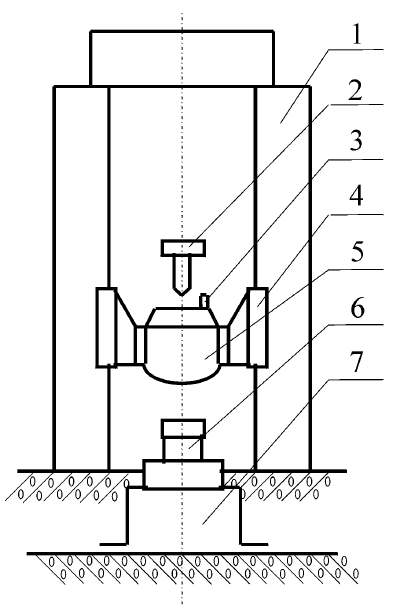
\includegraphics[width=4cm]{cn_100t.png} \\
    1.立柱 2.提升释放机构 3.标准冲击加速度计 \\
    4.导轨 5.重锤 6.被校力传感器 7.底座 \\
  \bicaption[出现在插图索引中]
    {单个图形示例\cite{he1999}。如果表格的标题很长,那么在表格索引中就会很不美观。可
      以在前面用中括号写一个简短的标题,这个标题会出现在索引中。}
    {Stay hungry, stay foolish.}
 \label{fig:cn_100t}
\end{figure}

Lorem ipsum dolor sit amet, consectetur adipisici elit, sed do eiusmod tempor
incididunt ut labore et dolore magna aliqua. Ut enim ad minim veniam, quis
nostrud exercitation ullamco laboris nisi ut aliquip ex ea commodo consequat.
Duis aute irure dolor in reprehenderit in voluptate velit esse cillum dolore eu
fugiat nulla pariatur. Excepteur sint occaecat cupidatat non proident, sunt in
culpa qui officia deserunt mollit anim id est laborum.

\subsection{多个图形}

简单插入多个图形的例子如图~\ref{fig:SRR} 所示。这两个水平并列放置的子图共用一个
图形计数器,没有各自的子图题。

\begin{figure}[!htp]
  \centering
  
\includegraphics[height=2cm]{bupt_badge.pdf}
  \hspace{1cm}
  
\includegraphics[height=2cm]{bupt_badge.pdf}
  \bicaption{中文题图}{English caption}
  \label{fig:SRR}
\end{figure}

如果多个图形相互独立,并不共用一个图形计数器,那么用 \texttt{minipage} 或者
\texttt{parbox} 就可以,如图~\ref{fig:parallel1} 与图~\ref{fig:parallel2}。

\begin{figure}[!htp]
\begin{minipage}{0.48\textwidth}
  \centering
  
\includegraphics[height=1.5cm]{bupt_name.pdf}
  \caption{并排第一个图}
  \label{fig:parallel1}
\end{minipage}\hfill
\begin{minipage}{0.48\textwidth}
  \centering
  
\includegraphics[height=1.5cm]{bupt_name.pdf}
  \caption{并排第二个图}
  \label{fig:parallel2}
\end{minipage}
\end{figure}

Lorem ipsum dolor sit amet, consectetur adipisici elit, sed do eiusmod tempor
incididunt ut labore et dolore magna aliqua. Ut enim ad minim veniam, quis
nostrud exercitation ullamco laboris nisi ut aliquip ex ea commodo consequat.
Duis aute irure dolor in reprehenderit in voluptate velit esse cillum dolore eu
fugiat nulla pariatur. Excepteur sint occaecat cupidatat non proident, sunt in
culpa qui officia deserunt mollit anim id est laborum.

如果要为共用一个计数器的多个子图添加子图题,建议使用较新的 \pkg{subcaption}宏
包,不建议使用 \pkg{subfigure} 或 \pkg{subfig} 等宏包。

推荐使用 \pkg{subcaption} 宏包的 \cs{subcaptionbox} 并排子图,子图题置于子图之
下,子图号用 a)、b) 等表示。也可以使用 \pkg{subcaption} 宏包的 \cs{subcaption}
(放在 minipage中,用法同 \cs{caption})。

搭配 \pkg{bicaption} 宏包时,可以启用 \cs{subcaptionbox} 和 \cs{subcaption} 的双
语变种 \cs{bisubcaptionbox} 和 \cs{bisubcaption},如图~\ref{fig:bisubcaptionbox}
所示。

\begin{figure}[!hbtp]
  \centering
  \bisubcaptionbox{$R_3 = 1.5\text{mm}$ 时轴承的压力分布云图}%
                  {Pressure contour of bearing when $R_3 = 1.5\text{mm}$}%
                  [6.4cm]{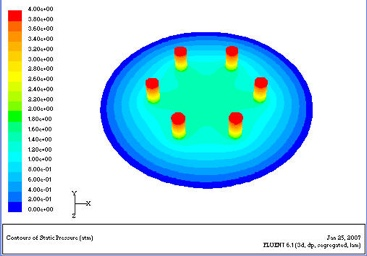
\includegraphics[height=2.5cm]{pressure15.jpg}}
  \hspace{1cm}
  \bisubcaptionbox{$R_3 = 2.5\text{mm}$ 时轴承的压力分布云图}%
                  {Pressure contour of bearing when $R_3 = 2.5\text{mm}$}%
                  [6.4cm]{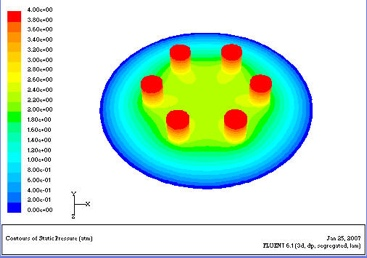
\includegraphics[height=2.5cm]{/pressure25.jpg}}
  \bicaption{包含子图题的范例(使用 subcaptionbox)}
            {Example with subcaptionbox}
  \label{fig:bisubcaptionbox}
\end{figure}

\pkg{subcaption} 宏包也提供了 \pkg{subfigure} 和 \pkg{subtable} 环境,如
图~\ref{fig:subfigure}。

\begin{figure}[!htp]
  \centering
  \begin{subfigure}{0.3\textwidth}
    \centering
    
\includegraphics[height=2cm]{bupt_badge.pdf}
    \caption{校徽}
  \end{subfigure}
  \hspace{1cm}
  \begin{subfigure}{0.4\textwidth}
    \centering
    
\includegraphics[height=1.5cm]{bupt_name.pdf}
    \caption{校名。注意这个图略矮些,subfigure 中同一行的子图在顶端对齐。}
  \end{subfigure}
  \caption{包含子图题的范例(使用 subfigure)}
  \label{fig:subfigure}
\end{figure}

Lorem ipsum dolor sit amet, consectetur adipisici elit, sed do eiusmod tempor
incididunt ut labore et dolore magna aliqua. Ut enim ad minim veniam, quis
nostrud exercitation ullamco laboris nisi ut aliquip ex ea commodo consequat.
Duis aute irure dolor in reprehenderit in voluptate velit esse cillum dolore eu
fugiat nulla pariatur. Excepteur sint occaecat cupidatat non proident, sunt in
culpa qui officia deserunt mollit anim id est laborum.

\section{表格}

\subsection{基本表格}

编排表格应简单明了,表达一致,明晰易懂,表文呼应、内容一致。表题置于表上,研究生
学位论文可以用中、英文两种文字居中排写,中文在上,也可以只用中文。

表格的编排建议采用国际通行的三线表\footnote{三线表,以其形式简洁、功能分明、阅读
方便而在科技论文中被推荐使用。三线表通常只有 3 条线,即顶线、底线和栏目线,没有
竖线。}。三线表可以使用 \pkg{booktabs} 提供的 \cs{toprule}、\cs{midrule} 和
\cs{bottomrule}。它们与 \pkg{longtable} 能很好的配合使用。

\begin{table}[!hpt]
  \caption[一个颇为标准的三线表]{一个颇为标准的三线表\footnotemark}
  \label{tab:firstone}
  \centering
  \begin{tabular}{@{}llr@{}} \toprule
    \multicolumn{2}{c}{Item} \\ \cmidrule(r){1-2}
    Animal & Description & Price (\$)\\ \midrule
    Gnat  & per gram  & 13.65 \\
          & each      & 0.01 \\
    Gnu   & stuffed   & 92.50 \\
    Emu   & stuffed   & 33.33 \\
    Armadillo & frozen & 8.99 \\ \bottomrule
  \end{tabular}
\end{table}
\footnotetext{这个例子来自
  \href{https://mirrors.sjtug.sjtu.edu.cn/ctan/macros/latex/contrib/booktabs/booktabs.pdf}%
  {《Publication quality tables in LaTeX》}(\pkg{booktabs} 宏包的文档)。这也是
  一个在表格中使用脚注的例子,请留意与 \pkg{threeparttable} 实现的效果有何不
  同。}

\subsection{复杂表格}

我们经常会在表格下方标注数据来源,或者对表格里面的条目进行解释。可以用
\pkg{threeparttable} 实现带有脚注的表格,如表~\ref{tab:footnote}。

\begin{table}[!htpb]
  \bicaption{一个带有脚注的表格的例子}{A Table with footnotes}
  \label{tab:footnote}
  \centering
  \begin{threeparttable}[b]
     \begin{tabular}{ccd{4}cccc}
      \toprule
      \multirow{2}*{total} & \multicolumn{2}{c}{20\tnote{a}} & \multicolumn{2}{c}{40} & \multicolumn{2}{c}{60} \\
      \cmidrule(lr){2-3}\cmidrule(lr){4-5}\cmidrule(lr){6-7}
      & www & \multicolumn{1}{c}{k} & www & k & www & k \\ % 使用说明符 d 的列会自动进入数学模式,使用 \multicolumn 对文字表头做特殊处理
      \midrule
      & $\underset{(2.12)}{4.22}$ & 120.0140\tnote{b} & 333.15 & 0.0411 & 444.99 & 0.1387 \\
      & 168.6123 & 10.86 & 255.37 & 0.0353 & 376.14 & 0.1058 \\
      & 6.761    & 0.007 & 235.37 & 0.0267 & 348.66 & 0.1010 \\
      \bottomrule
    \end{tabular}
    \begin{tablenotes}
    \item [a] the first note.% or \item [a]
    \item [b] the second note.% or \item [b]
    \end{tablenotes}
  \end{threeparttable}
\end{table}

Lorem ipsum dolor sit amet, consectetur adipisici elit, sed do eiusmod tempor
incididunt ut labore et dolore magna aliqua. Ut enim ad minim veniam, quis
nostrud exercitation ullamco laboris nisi ut aliquip ex ea commodo consequat.
Duis aute irure dolor in reprehenderit in voluptate velit esse cillum dolore eu
fugiat nulla pariatur. Excepteur sint occaecat cupidatat non proident, sunt in
culpa qui officia deserunt mollit anim id est laborum.

如某个表需要转页接排,可以用 \pkg{longtable} 实现。接排时表题省略,表头应重复书
写,并在右上方写“续表 xx”,如表~\ref{tab:performance}。

\begin{longtable}[c]{c*{6}{r}}
  \bicaption{实验数据}{Experimental data}
  \label{tab:performance} \\
  \toprule
  测试程序 & \multicolumn{1}{c}{正常运行} & \multicolumn{1}{c}{同步}
    & \multicolumn{1}{c}{检查点} & \multicolumn{1}{c}{卷回恢复}
    & \multicolumn{1}{c}{进程迁移} & \multicolumn{1}{c}{检查点} \\
   & \multicolumn{1}{c}{时间 (s)} & \multicolumn{1}{c}{时间 (s)}
    & \multicolumn{1}{c}{时间 (s)} & \multicolumn{1}{c}{时间 (s)}
    & \multicolumn{1}{c}{时间 (s)} &  文件(KB)\\
  \midrule
  \endfirsthead
  \multicolumn{7}{r}{续表~\thetable} \\
  \toprule
  测试程序 & \multicolumn{1}{c}{正常运行} & \multicolumn{1}{c}{同步}
    & \multicolumn{1}{c}{检查点} & \multicolumn{1}{c}{卷回恢复}
    & \multicolumn{1}{c}{进程迁移} & \multicolumn{1}{c}{检查点} \\
   & \multicolumn{1}{c}{时间 (s)} & \multicolumn{1}{c}{时间 (s)}
    & \multicolumn{1}{c}{时间 (s)} & \multicolumn{1}{c}{时间 (s)}
    & \multicolumn{1}{c}{时间 (s)}&  文件(KB)\\
  \midrule
  \endhead
  \hline
  \multicolumn{7}{r}{续下页}
  \endfoot
  \endlastfoot
  CG.A.2 & 23.05 & 0.002 & 0.116 & 0.035 & 0.589 & 32491 \\
  CG.A.4 & 15.06 & 0.003 & 0.067 & 0.021 & 0.351 & 18211 \\
  CG.A.8 & 13.38 & 0.004 & 0.072 & 0.023 & 0.210 & 9890 \\
  CG.B.2 & 867.45 & 0.002 & 0.864 & 0.232 & 3.256 & 228562 \\
  CG.B.4 & 501.61 & 0.003 & 0.438 & 0.136 & 2.075 & 123862 \\
  CG.B.8 & 384.65 & 0.004 & 0.457 & 0.108 & 1.235 & 63777 \\
  MG.A.2 & 112.27 & 0.002 & 0.846 & 0.237 & 3.930 & 236473 \\
  MG.A.4 & 59.84 & 0.003 & 0.442 & 0.128 & 2.070 & 123875 \\
  MG.A.8 & 31.38 & 0.003 & 0.476 & 0.114 & 1.041 & 60627 \\
  MG.B.2 & 526.28 & 0.002 & 0.821 & 0.238 & 4.176 & 236635 \\
  MG.B.4 & 280.11 & 0.003 & 0.432 & 0.130 & 1.706 & 123793 \\
  MG.B.8 & 148.29 & 0.003 & 0.442 & 0.116 & 0.893 & 60600 \\
  LU.A.2 & 2116.54 & 0.002 & 0.110 & 0.030 & 0.532 & 28754 \\
  LU.A.4 & 1102.50 & 0.002 & 0.069 & 0.017 & 0.255 & 14915 \\
  LU.A.8 & 574.47 & 0.003 & 0.067 & 0.016 & 0.192 & 8655 \\
  LU.B.2 & 9712.87 & 0.002 & 0.357 & 0.104 & 1.734 & 101975 \\
  LU.B.4 & 4757.80 & 0.003 & 0.190 & 0.056 & 0.808 & 53522 \\
  LU.B.8 & 2444.05 & 0.004 & 0.222 & 0.057 & 0.548 & 30134 \\
  EP.A.2 & 123.81 & 0.002 & 0.010 & 0.003 & 0.074 & 1834 \\
  EP.A.4 & 61.92 & 0.003 & 0.011 & 0.004 & 0.073 & 1743 \\
  EP.A.8 & 31.06 & 0.004 & 0.017 & 0.005 & 0.073 & 1661 \\
  EP.B.2 & 495.49 & 0.001 & 0.009 & 0.003 & 0.196 & 2011 \\
  EP.B.4 & 247.69 & 0.002 & 0.012 & 0.004 & 0.122 & 1663 \\
  EP.B.8 & 126.74 & 0.003 & 0.017 & 0.005 & 0.083 & 1656 \\
  SP.A.2 & 123.81 & 0.002 & 0.010 & 0.003 & 0.074 & 1854 \\
  SP.A.4 & 51.92 & 0.003 & 0.011 & 0.004 & 0.073 & 1543 \\
  SP.A.8 & 31.06 & 0.004 & 0.017 & 0.005 & 0.073 & 1671 \\
  SP.B.2 & 495.49 & 0.001 & 0.009 & 0.003 & 0.196 & 2411 \\
  SP.B.4 & 247.69 & 0.002 & 0.014 & 0.006 & 0.152 & 2653 \\
  SP.B.8 & 126.74 & 0.003 & 0.017 & 0.005 & 0.082 & 1755 \\
  \bottomrule
\end{longtable}

\section{算法环境}

算法环境可以使用 \pkg{algorithms} 宏包或者较新的 \pkg{algorithm2e} 实现。
算法~\ref{algo:algorithm} 是一个使用 \pkg{algorithm2e} 的例子。关于排版算法环境
的具体方法,请阅读相关宏包的官方文档。

\begin{algorithm}[htb]
  \caption{算法示例}
  \label{algo:algorithm}
  \small
  \SetAlgoLined
  \KwData{this text}
  \KwResult{how to write algorithm with \LaTeXe }

  initialization\;
  \While{not at end of this document}{
    read current\;
    \eIf{understand}{
      go to next section\;
      current section becomes this one\;
    }{
      go back to the beginning of current section\;
    }
  }
\end{algorithm}

\section{代码环境}

我们可以在论文中插入算法,但是不建议插入大段的代码。如果确实需要插入代码,建议使
用 \pkg{listings} 宏包。

\begin{codeblock}[language=C]
#include <stdio.h>
#include <unistd.h>
#include <sys/types.h>
#include <sys/wait.h>

int main() {
  pid_t pid;

  switch ((pid = fork())) {
  case -1:
    printf("fork failed\n");
    break;
  case 0:
    /* child calls exec */
    execl("/bin/ls", "ls", "-l", (char*)0);
    printf("execl failed\n");
    break;
  default:
    /* parent uses wait to suspend execution until child finishes */
    wait((int*)0);
    printf("is completed\n");
    break;
  }

  return 0;
}
\end{codeblock}

% !TEX root = ../thesis.tex

\chapter{数学与引用文献的标注}

\section{数学}

\subsection{数字和单位}

宏包 \pkg{siunitx} 提供了更好的数字和单位支持:
\begin{itemize}
  \item \num{12345.67890}
  \item \num{1+-2i}
  \item \num{.3e45}
  \item \num{1.654 x 2.34 x 3.430}
  \item \si{kg.m.s^{-1}}
  \item \si{\micro\meter} $\si{\micro\meter}$
  \item \si{\ohm} $\si{\ohm}$
  \item \numlist{10;20}
  \item \numlist{10;20;30}
  \item \SIlist{0.13;0.67;0.80}{\milli\metre}
  \item \numrange{10}{20}
  \item \SIrange{10}{20}{\degreeCelsius}
\end{itemize}

\subsection{数学符号和公式}

微分符号 $\dif$ 应使用正体,本模板提供了 \cs{dif} 命令。除此之外,模板还提供了一
些命令方便使用:
\begin{itemize}
  \item 圆周率 $\uppi$:\verb|\uppi|
  \item 自然对数的底 $\upe$:\verb|\upe|
  \item 虚数单位 $\upi$, $\upj$:\verb|\upi| \verb|\upj|
\end{itemize}

公式应另起一行居中排版。公式后应注明编号,按章顺序编排,编号右端对齐。
\begin{equation}
  \upe^{\upi\uppi} + 1 = 0
\end{equation}
\begin{equation}
  \frac{\dif^2 u}{\dif t^2} = \int f(x) \dif x
\end{equation}

公式较长时最好在等号“$=$”处转行。
\begin{align}
    & I (X_3; X_4) - I (X_3; X_4 \mid X_1) - I (X_3; X_4 \mid X_2) \nonumber \\
  = & [I (X_3; X_4) - I (X_3; X_4 \mid X_1)] - I (X_3; X_4 \mid \tilde{X}_2) \\
  = & I (X_1; X_3; X_4) - I (X_3; X_4 \mid \tilde{X}_2)
\end{align}

如果在等号处转行难以实现,也可在 $+$、$-$、$\times$、$\div$运算符号处转行,转行
时运算符号仅书写于转行式前,不重复书写。
\begin{multline}
  \frac{1}{2} \Delta (f_{ij} f^{ij}) =
    2 \left(\sum_{i<j} \chi_{ij}(\sigma_{i} - \sigma_{j})^{2}
    + f^{ij} \nabla_{j} \nabla_{i} (\Delta f) \right. \\
  \left. + \nabla_{k} f_{ij} \nabla^{k} f^{ij} +
    f^{ij} f^{k} \left[2\nabla_{i}R_{jk}
    - \nabla_{k} R_{ij} \right] \vphantom{\sum_{i<j}} \right)
\end{multline}

\subsection{定理环境}

示例文件中使用 \pkg{ntheorem} 宏包配置了定理、引理和证明等环境。用户也可以使用
\pkg{amsthm} 宏包。

这里举一个“定理”和“证明”的例子。
\begin{theorem}[留数定理]
\label{thm:res}
  假设 $U$ 是复平面上的一个单连通开子集,$a_1, \ldots, a_n$ 是复平面上有限个点,
  $f$ 是定义在 $U \backslash \{a_1, \ldots, a_n\}$ 上的全纯函数,如果 $\gamma$
  是一条把 $a_1, \ldots, a_n$ 包围起来的可求长曲线,但不经过任何一个 $a_k$,并且
  其起点与终点重合,那么:

  \begin{equation}
    \label{eq:res}
    \ointop_\gamma f(z)\, \dif z = 2\uppi \upi \sum_{k=1}^n \operatorname{I}(\gamma, a_k) \operatorname{Res}(f, a_k)
  \end{equation}

  如果 $\gamma$ 是若尔当曲线,那么 $\operatorname{I}(\gamma, a_k) = 1$,因此:

  \begin{equation}
    \label{eq:resthm}
    \ointop_\gamma f(z)\, \dif z = 2\uppi \upi \sum_{k=1}^n \operatorname{Res}(f, a_k)
  \end{equation}

  在这里,$\operatorname{Res}(f, a_k)$ 表示 $f$ 在点 $a_k$ 的留数,
  $\operatorname{I}(\gamma, a_k)$ 表示 $\gamma$ 关于点 $a_k$ 的卷绕数。卷绕数是
  一个整数,它描述了曲线 $\gamma$ 绕过点 $a_k$ 的次数。如果 $\gamma$ 依逆时针方
  向绕着 $a_k$ 移动,卷绕数就是一个正数,如果 $\gamma$ 根本不绕过 $a_k$,卷绕数
  就是零。

  定理~\ref{thm:res} 的证明。

  \begin{proof}
    首先,由……

    其次,……

    所以……
  \end{proof}
\end{theorem}

\section{引用文献的标注}

按照教务处的要求,参考文献外观应符合国标 GB/T 7714 的要求。模版使用 \BibLaTeX\
配合 \pkg{biblatex-gb7714-2015} 样式包
\footnote{\url{https://www.ctan.org/pkg/biblatex-gb7714-2015}}
控制参考文献的输出样式,后端采用 \pkg{biber} 管理文献。

请注意 \pkg{biblatex-gb7714-2015} 宏包 2016 年 9 月才加入 CTAN,如果你使用的
\TeX\ 系统版本较旧,可能没有包含 \pkg{biblatex-gb7714-2015} 宏包,需要手动安装。
\BibLaTeX\ 与 \pkg{biblatex-gb7714-2015} 目前在活跃地更新,为避免一些兼容性问
题,推荐使用较新的版本。

正文中引用参考文献时,使用 \verb|\cite{key1,key2,key3...}| 可以产生“上标引用的
参考文献”,如 \cite{Meta_CN,chen2007act,DPMG}。使用
\verb|\parencite{key1,key2,key3...}| 则可以产生水平引用的参考文献,例如
\parencite{JohnD,zhubajie,IEEE-1363}。请看下面的例子,将会穿插使用水平的和上标的
参考文献:关于书的\parencite{Meta_CN,JohnD,IEEE-1363},关于期刊的
\cite{chen2007act,chen2007ewi},会议论文 \parencite{DPMG,kocher99,cnproceed},硕
士学位论文\parencite{zhubajie,metamori2004},博士学位论文
\cite{shaheshang,FistSystem01,bai2008},标准文件 \parencite{IEEE-1363},技术报告
\cite{NPB2},电子文献 \parencite{xiaoyu2001, CHRISTINE1998},用户手册
\parencite{RManual}。

当需要将参考文献条目加入到文献表中但又不在正文中引用,可以使用
\verb|\nocite{key1,key2,key3...}|。使用 \verb|\nocite{*}| 可以将参考文献数据库中
的所有条目加入到文献表中。

% !TEX root = ../thesis.tex

\begin{summary}
这里是全文总结内容。

2015 年 2 月 28 日,中央在北京召开全国精神文明建设工作表彰暨学雷锋志愿服务大会,
公布全国文明城市(区)、文明村镇、文明单位名单。上海交通大学荣获全国文明单位称
号。

全国文明单位这一荣誉是对交大人始终高度重视文明文化工作的肯定,是对交大长期以来文
明创建工作成绩的褒奖。在学校党委、文明委的领导下,交大坚持将文明创建工作纳入学校
建设世界一流大学的工作中,全体师生医护员工群策群力、积极开拓,落实国家和上海市有
关文明创建的各项要求,以改革创新、科学发展为主线,以质量提升为目标,聚焦文明创建
工作出现的重点和难点,优化文明创建工作机制,传播学校良好形象,提升社会美誉度,显
著增强学校软实力。2007 至 2012 年间,上海交大连续三届荣获“上海市文明单位”称
号,成为创建全国文明单位的新起点。

上海交大自启动争创全国文明单位工作以来,凝魂聚气、改革创新,积极培育和践行社会主
义核心价值观。坚持统筹兼顾、多措并举,将争创全国文明单位与学校各项中心工作紧密结
合,着力构建学校文明创建新格局,不断提升师生医护员工文明素养,以“冲击世界一流大
学汇聚强大精神动力”为指导思想,以“聚焦改革、多元推进、以评促建、丰富内涵、彰显
特色”为工作原则,并由全体校领导群策领衔“党的建设深化、思想教育深入、办学成绩显
著、大学文化丰富、校园环境优化、社会责任担当”六大板块共 28 项重点突破工作,全面
展现近年来交大文明创建工作的全貌和成就。

进入新阶段,学校将继续开拓文明创建工作新格局,不断深化工作理念和工作实践,创新工
作载体、丰富活动内涵、凸显创建成效,积极服务于学校各项中心工作和改革发展的大局
面,在上级党委、文明委的关心下,在学校党委的直接领导下,与时俱进、开拓创新,为深
化内涵建设、加快建成世界一流大学、推动国家进步和社会发展而努力奋斗!

上海交通大学医学院附属仁济医院也获得全国文明单位称号。
\end{summary}


% 使用英文字母对附录编号
\appendix

% 附录内容,本科学位论文可以用翻译的文献替代。
% !TEX root = ../thesis.tex

\chapter{Maxwell Equations}

选择二维情况,有如下的偏振矢量:
\begin{subequations}
  \begin{align}
    {\bf E} &= E_z(r, \theta) \hat{\bf z} \\
    {\bf H} &= H_r(r, \theta) \hat{\bf r} + H_\theta(r, \theta) \hat{\bm\theta}
  \end{align}
\end{subequations}
对上式求旋度:
\begin{subequations}
  \begin{align}
    \nabla \times {\bf E} &= \frac{1}{r} \frac{\partial E_z}{\partial\theta}
      \hat{\bf r} - \frac{\partial E_z}{\partial r} \hat{\bm\theta} \\
    \nabla \times {\bf H} &= \left[\frac{1}{r} \frac{\partial}{\partial r}
      (r H_\theta) - \frac{1}{r} \frac{\partial H_r}{\partial\theta} \right]
      \hat{\bf z}
  \end{align}
\end{subequations}
因为在柱坐标系下,$\overline{\overline\mu}$ 是对角的,所以 Maxwell 方程组中电场
$\bf E$ 的旋度:
\begin{subequations}
  \begin{align}
    & \nabla \times {\bf E} = \upi \omega {\bf B} \\
    & \frac{1}{r} \frac{\partial E_z}{\partial\theta} \hat{\bf r} -
      \frac{\partial E_z}{\partial r}\hat{\bm\theta} = \upi \omega \mu_r H_r
      \hat{\bf r} + \upi \omega \mu_\theta H_\theta \hat{\bm\theta}
  \end{align}
\end{subequations}
所以 $\bf H$ 的各个分量可以写为:
\begin{subequations}
  \begin{align}
    H_r &= \frac{1}{\upi \omega \mu_r} \frac{1}{r}
      \frac{\partial E_z}{\partial\theta} \\
    H_\theta &= -\frac{1}{\upi \omega \mu_\theta}
      \frac{\partial E_z}{\partial r}
  \end{align}
\end{subequations}
同样地,在柱坐标系下,$\overline{\overline\epsilon}$ 是对角的,所以 Maxwell 方程
组中磁场 $\bf H$ 的旋度:
\begin{subequations}
  \begin{align}
    & \nabla \times {\bf H} = -\upi \omega {\bf D} \\
    & \left[\frac{1}{r} \frac{\partial}{\partial r}(r H_\theta) - \frac{1}{r}
      \frac{\partial H_r}{\partial\theta} \right] \hat{\bf z} = -\upi \omega
      {\overline{\overline\epsilon}} {\bf E} = -\upi \omega \epsilon_z E_z
      \hat{\bf z} \\
    & \frac{1}{r} \frac{\partial}{\partial r}(r H_\theta) - \frac{1}{r}
      \frac{\partial H_r}{\partial\theta} = -\upi \omega \epsilon_z E_z
  \end{align}
\end{subequations}
由此我们可以得到关于 $E_z$ 的波函数方程:
\begin{equation}
  \frac{1}{\mu_\theta \epsilon_z} \frac{1}{r} \frac{\partial}{\partial r}
  \left(r \frac{\partial E_z}{\partial r} \right) + \frac{1}{\mu_r \epsilon_z}
  \frac{1}{r^2} \frac{\partial^2E_z}{\partial\theta^2} +\omega^2 E_z = 0
\end{equation}

% !TEX root = ../thesis.tex

\chapter{绘制流程图}

图~\ref{fig:flow_chart} 是一张流程图示意。使用 \pkg{tikz} 环境,搭配四种预定义节
点(\verb+startstop+、\verb+process+、\verb+decision+和\verb+io+),可以容易地绘
制出流程图。

\begin{figure}[!htp]
  \centering
  \resizebox{6cm}{!}{\begin{tikzpicture}[node distance=2cm]
    \node (pic) [startstop] {待测图片};
    \node (bg) [io, below of=pic] {读取背景};
    \node (pair) [process, below of=bg] {匹配特征点对};
    \node (threshold) [decision, below of=pair, yshift=-0.5cm] {多于阈值};
    \node (clear) [decision, right of=threshold, xshift=3cm] {清晰?};
    \node (capture) [process, right of=pair, xshift=3cm, yshift=0.5cm] {重采};
    \node (matrix_p) [process, below of=threshold, yshift=-0.8cm] {透视变换矩阵};
    \node (matrix_a) [process, right of=matrix_p, xshift=3cm] {仿射变换矩阵};
    \node (reg) [process, below of=matrix_p] {图像修正};
    \node (return) [startstop, below of=reg] {配准结果};
     
    %连接具体形状
    \draw [arrow](pic) -- (bg);
    \draw [arrow](bg) -- (pair);
    \draw [arrow](pair) -- (threshold);

    \draw [arrow](threshold) -- node[anchor=south] {否} (clear);

    \draw [arrow](clear) -- node[anchor=west] {否} (capture);
    \draw [arrow](capture) |- (pic);
    \draw [arrow](clear) -- node[anchor=west] {是} (matrix_a);
    \draw [arrow](matrix_a) |- (reg);

    \draw [arrow](threshold) -- node[anchor=east] {是} (matrix_p);
    \draw [arrow](matrix_p) -- (reg);
    \draw [arrow](reg) -- (return);
\end{tikzpicture}
}
  \bicaption{绘制流程图效果}{Flow chart}
  \label{fig:flow_chart}
\end{figure}


% 文后无编号部分
\backmatter

% 参考资料
\printbibliography[heading=bibintoc]

% 用于盲审的论文需隐去致谢、发表论文、参与项目、申请专利、简历

% 致谢
% !TEX root = ../thesis.tex

%TC:ignore

\begin{acknowledgements}
  感谢那位最先制作出博士学位论文 \LaTeX 模板的交大物理系同学!

  感谢 William Wang 同学对模板移植做出的巨大贡献!

  感谢 \href{https://github.com/weijianwen}{@weijianwen} 学长一直以来的开发和维
  护工作!

  感谢 \href{https://github.com/sjtug}{@sjtug} 以及
   \href{https://github.com/dyweb}{@dyweb} 对 0.9.5 之后版本的开发和维护工作!

  感谢所有为模板贡献过代码的同学们, 以及所有测试和使用模板的各位同学!

  感谢 \LaTeX 和 \href{https://github.com/sjtug/SJTUThesis}{\buptthesis},帮我节
  省了不少时间。
\end{acknowledgements}

%TC:endignore


% 发表论文、参与项目、申请专利、简历
% 盲审论文中,发表学术论文及参与科研情况等仅以第几作者注明即可,不要出现作者或他人姓名
%% !TEX root = ../thesis.tex

%TC:ignore

\begin{publications}
  \item Chen H, Chan C~T. Acoustic cloaking in three dimensions using acoustic metamaterials[J]. Applied Physics Letters, 2007, 91:183518.
  \item Chen H, Wu B~I, Zhang B, et al. Electromagnetic Wave Interactions with a Metamaterial Cloak[J]. Physical Review Letters, 2007, 99(6):63903.
\end{publications}

\begin{publications*}
  \item 第一作者. 中文核心期刊论文, 2007.
  \item 第一作者. EI 国际会议论文, 2006.
\end{publications*}

%TC:endignore

%% !TEX root = ../thesis.tex

%TC:ignore

\begin{projects}
  \item 参与973项目子课题(2007年6月--2008年5月)
  \item 参与自然基金项目(2005年5月--2005年8月)
  \item 参与国防项目(2005年8月--2005年10月)
\end{projects}

\begin{projects*}
  \item 973项目“XXX”
  \item 自然基金项目“XXX”
  \item 国防项目“XXX”
\end{projects*}

%TC:endignore

%% !TEX root = ../thesis.tex

%TC:ignore

\begin{patents}
  \item 第一发明人,“永动机”,专利申请号202510149890.0
\end{patents}

\begin{patents*}
  \item 第一发明人,“永动机”,专利申请号XXXXXXXXXXXX.X
\end{patents*}

%TC:endignore

%% !TEX root = ../thesis.tex

%TC:ignore

\begin{resume}
  \subsection*{基本情况}
    某某,yyyy 年 mm 月生于 xxxx。

  \subsection*{教育背景}
  \begin{itemize}
    \item yyyy 年 mm 月至今,上海交通大学,博士研究生,xx 专业
    \item yyyy 年 mm 月至 yyyy 年 mm 月,上海交通大学,硕士研究生,xx 专业
    \item yyyy 年 mm 月至 yyyy 年 mm 月,上海交通大学,本科,xx 专业
  \end{itemize}

  \subsection*{研究兴趣}
    \LaTeX{} 排版

  \subsection*{联系方式}
  \begin{itemize}
    \item 地址: 上海市闵行区东川路 800 号,200240
    \item E-mail: \email{xxx@sjtu.edu.cn}
  \end{itemize}
\end{resume}

%TC:endignore


% 中文学士学位论文要求在最后有一个英文大摘要,单独编页码,英文学士学位论文不需要
% !TEX root = ../thesis.tex

\begin{bigabstract}
  An imperial edict issued in 1896 by Emperor Guangxu, established Nanyang
  Public School in Shanghai. The normal school, school of foreign studies,
  middle school and a high school were established. Sheng Xuanhuai, the person
  responsible for proposing the idea to the emperor, became the first president
  and is regarded as the founder of the university.

  During the 1930s, the university gained a reputation of nurturing top
  engineers. After the foundation of People's Republic, some faculties were
  transferred to other universities. A significant amount of its faculty were
  sent in 1956, by the national government, to Xi'an to help build up Xi'an Jiao
  Tong University in western China. Afterwards, the school was officially
  renamed Shanghai Jiao Tong University.

  Since the reform and opening up policy in China, SJTU has taken the lead in
  management reform of institutions for higher education, regaining its vigor
  and vitality with an unprecedented momentum of growth. SJTU includes five
  beautiful campuses, Xuhui, Minhang, Luwan Qibao, and Fahua, taking up an area
  of about 3,225,833 m2. A number of disciplines have been advancing towards the
  top echelon internationally, and a batch of burgeoning branches of learning
  have taken an important position domestically.

  Today SJTU has 31 schools (departments), 63 undergraduate programs, 250
  masters-degree programs, 203 Ph.D. programs, 28 post-doctorate programs, and
  11 state key laboratories and national engineering research centers.

  SJTU boasts a large number of famous scientists and professors, including 35
  academics of the Academy of Sciences and Academy of Engineering, 95 accredited
  professors and chair professors of the "Cheung Kong Scholars Program" and more
  than 2,000 professors and associate professors.

  Its total enrollment of students amounts to 35,929, of which 1,564 are
  international students. There are 16,802 undergraduates, and 17,563 masters
  and Ph.D. candidates. After more than a century of operation, Jiao Tong
  University has inherited the old tradition of "high starting points, solid
  foundation, strict requirements and extensive practice." Students from SJTU
  have won top prizes in various competitions, including ACM International
  Collegiate Programming Contest, International Mathematical Contest in Modeling
  and Electronics Design Contests. Famous alumni include Jiang Zemin, Lu Dingyi,
  Ding Guangen, Wang Daohan, Qian Xuesen, Wu Wenjun, Zou Taofen, Mao Yisheng,
  Cai Er, Huang Yanpei, Shao Lizi, Wang An and many more. More than 200 of the
  academics of the Chinese Academy of Sciences and Chinese Academy of
  Engineering are alumni of Jiao Tong University.
\end{bigabstract}


\end{document}
